\section{Interpretation of differential Higgs boson production cross sections}

\tk{TODO:
% 
Start with general motivation, include multiple possible uses of differential cross sections (e.g. constraining the gluon pdf using the rapidity distribution).
}


% ____________________________________________________________________________
\subsection{Simultaneous variations of \texorpdfstring{$\kappat$}{kt}, \texorpdfstring{$\kappab$}{kb}, and anomalous coupling \texorpdfstring{$\cg$}{cg}}

\tk{TODO:
Introduction of the theory, results when fitting it to data.
}


\subsubsection{Systematic uncertainties}

\tk{TODO:
Treat here how the scale variations are used, and explain the procedure to implement the bin-to-bin correlations in the likelihood.
% 
Note PDF uncertainties are not included.
% 
Refer back to this section for the kb/kc fits.
}


\subsubsection{Inclusive vs. differential measurements}

\tk{TODO:
Motivate the fits with coupling-dependent BRs and floating BRs.
% 
Refer back to this section for the kb/kc fits.
}


\subsubsection{Results}

\tk{TODO: Literal paper text now}

The fits are repeated in a way analogous to that of Section~\ref{sec:ResultsKappabKappac} but with $\kappat$, $\cg$, and $\kappab$ as the parameters of the fit, using the parametrization obtained from Ref.~\cite{Grazzini:2017szg}.
% 
The combined log-likelihood scan for $\kappat$ vs. $\cg$, assuming branching fractions that depend on the couplings, is shown in Fig.~\ref{fig:scans_kappatkappag_nominal} (left).
% 
The normalization of the spectrum is, by construction, equal to the SM normalization for the points $( \kappat = 1.0, \cg = 0.0 )$ and $( \kappat = 0.0, \cg \simeq 0.08 )$.
% 
The differential shape of the parametrization $s$ is calculated by normalizing the differential cross section to $1$:
% 
\begin{linenomath*}
\begin{equation}
    s_i(\kappat, \cg) =
        \frac
            {\sigma_i(\kappat, \cg)}
            {\sum_j \sigma_j(\kappat, \cg)}
    \,,
\end{equation}
\end{linenomath*}
% 
where $\sigma_i$ is the parametrization in bin $i$.
% 
Plugging in the expected parabolic dependence of $\sigma_i(\kappat, \cg)$
% 
reveals that the shape of the parametrization for $\kappat$/$\cg$ variations becomes a function of the ratio of the two couplings, $s_i(\frac{\kappat}{\cg})$.
% 
Thus any discrimination power in the radial direction with respect to the origin stems from constraints on the overall normalization, whereas discrimination in the angular direction stems from constraints on the shape of the distribution.
% 
The angular dependence of the log-likelihood function becomes apparent in Fig.~\ref{fig:scans_kappatkappag_nominal} (right), where the branching fractions are implemented as nuisance parameters with no prior constraint in the fit.
% 
Except at small values of the couplings, the constraint on the couplings depends on their ratio.
% 
The two symmetric sets of contours are due to a symmetry of the parametrization under $(\kappat,\,\cg) \, \to \, (-\kappat,\,-\cg)$.


\begin{figure}[hbtp]
  \begin{center}
    \ifbool{draftmode}{
        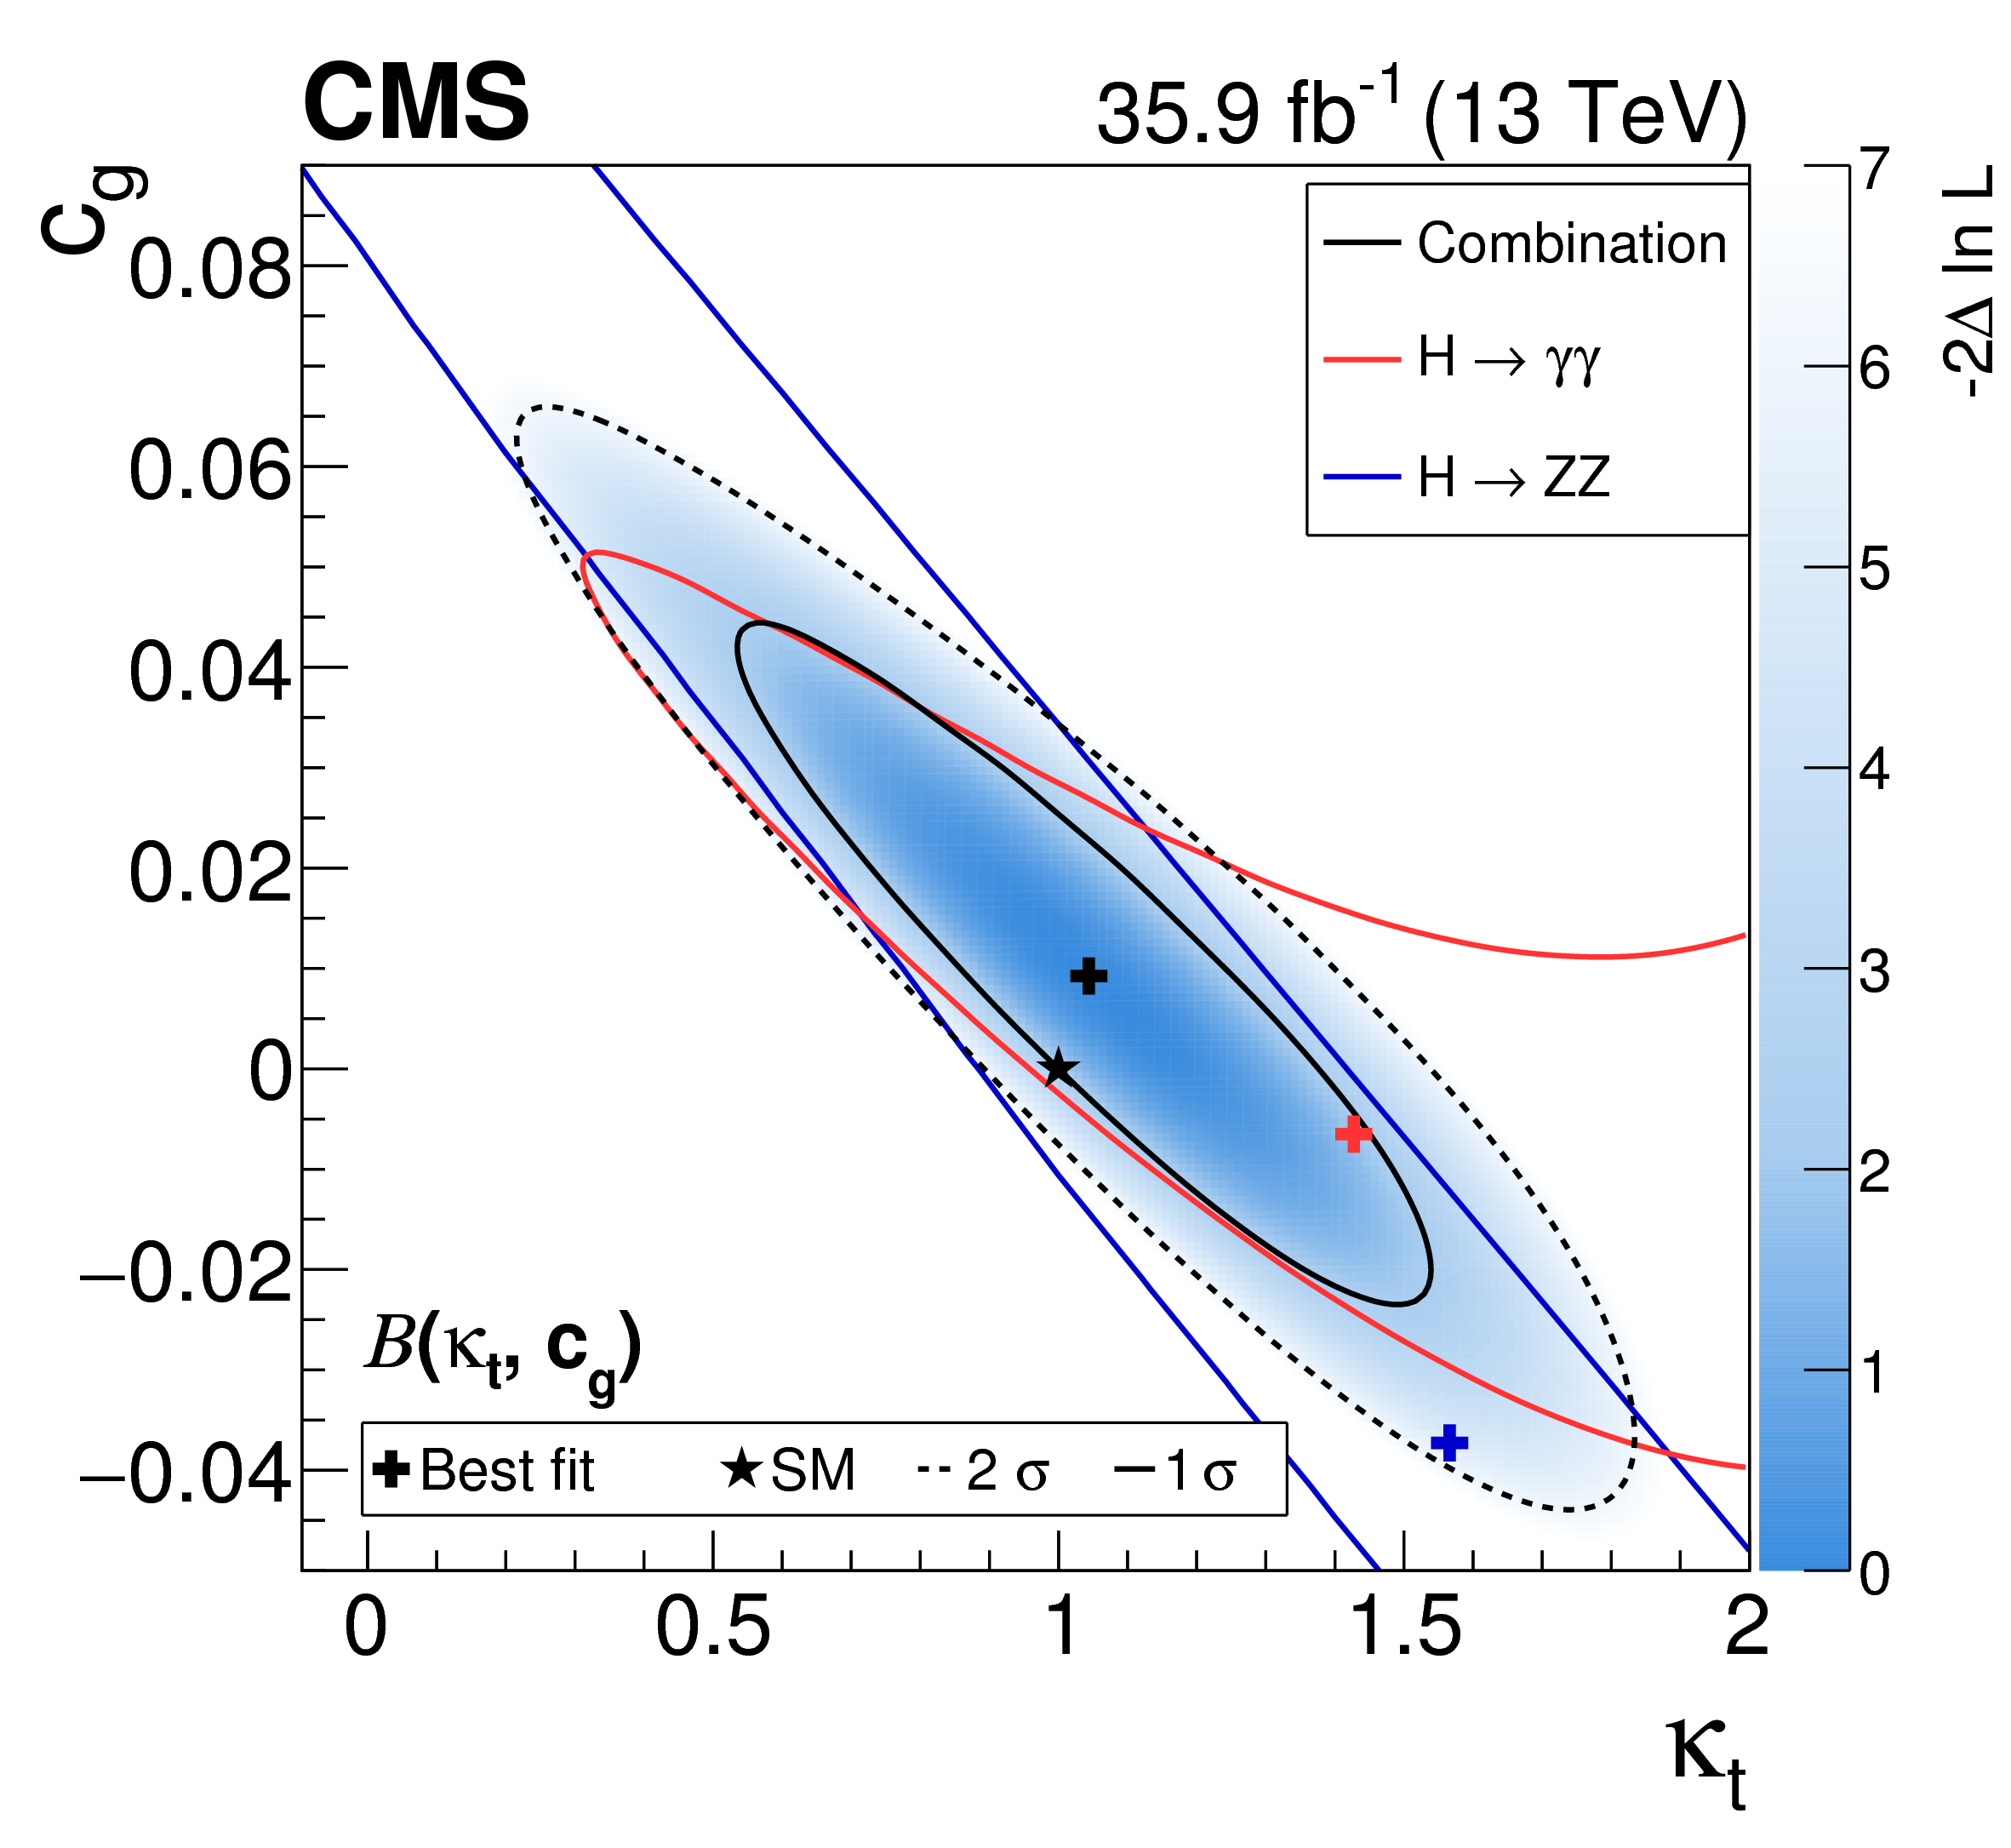
\includegraphics[width=0.49\linewidth]{img/interpretation/multicont_ktcg_couplingdependentBRs.png}
        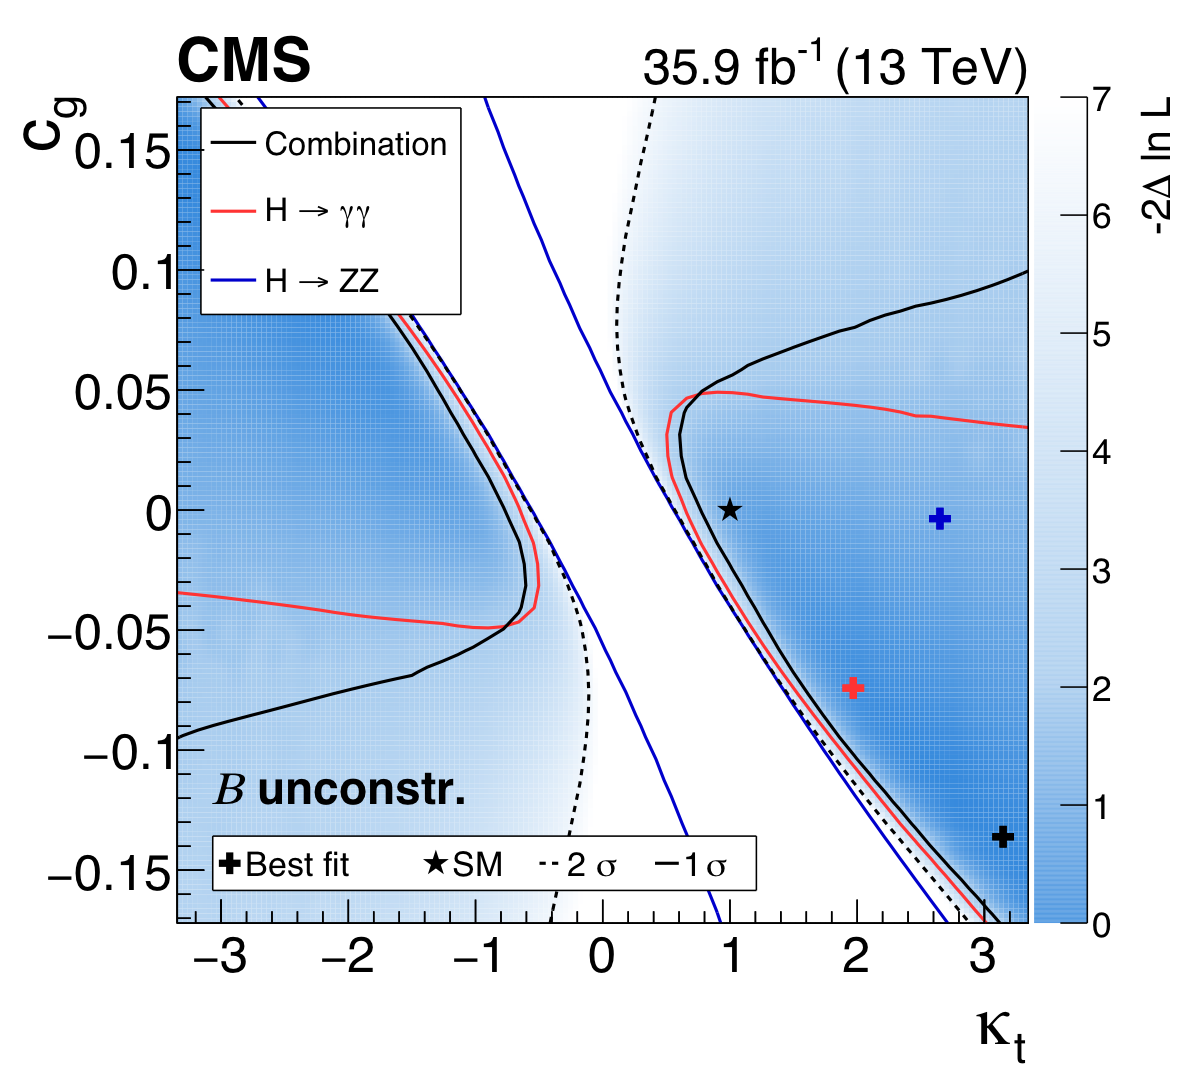
\includegraphics[width=0.49\linewidth]{img/interpretation/multicont_ktcg_floatingBRs.png}
        }{
        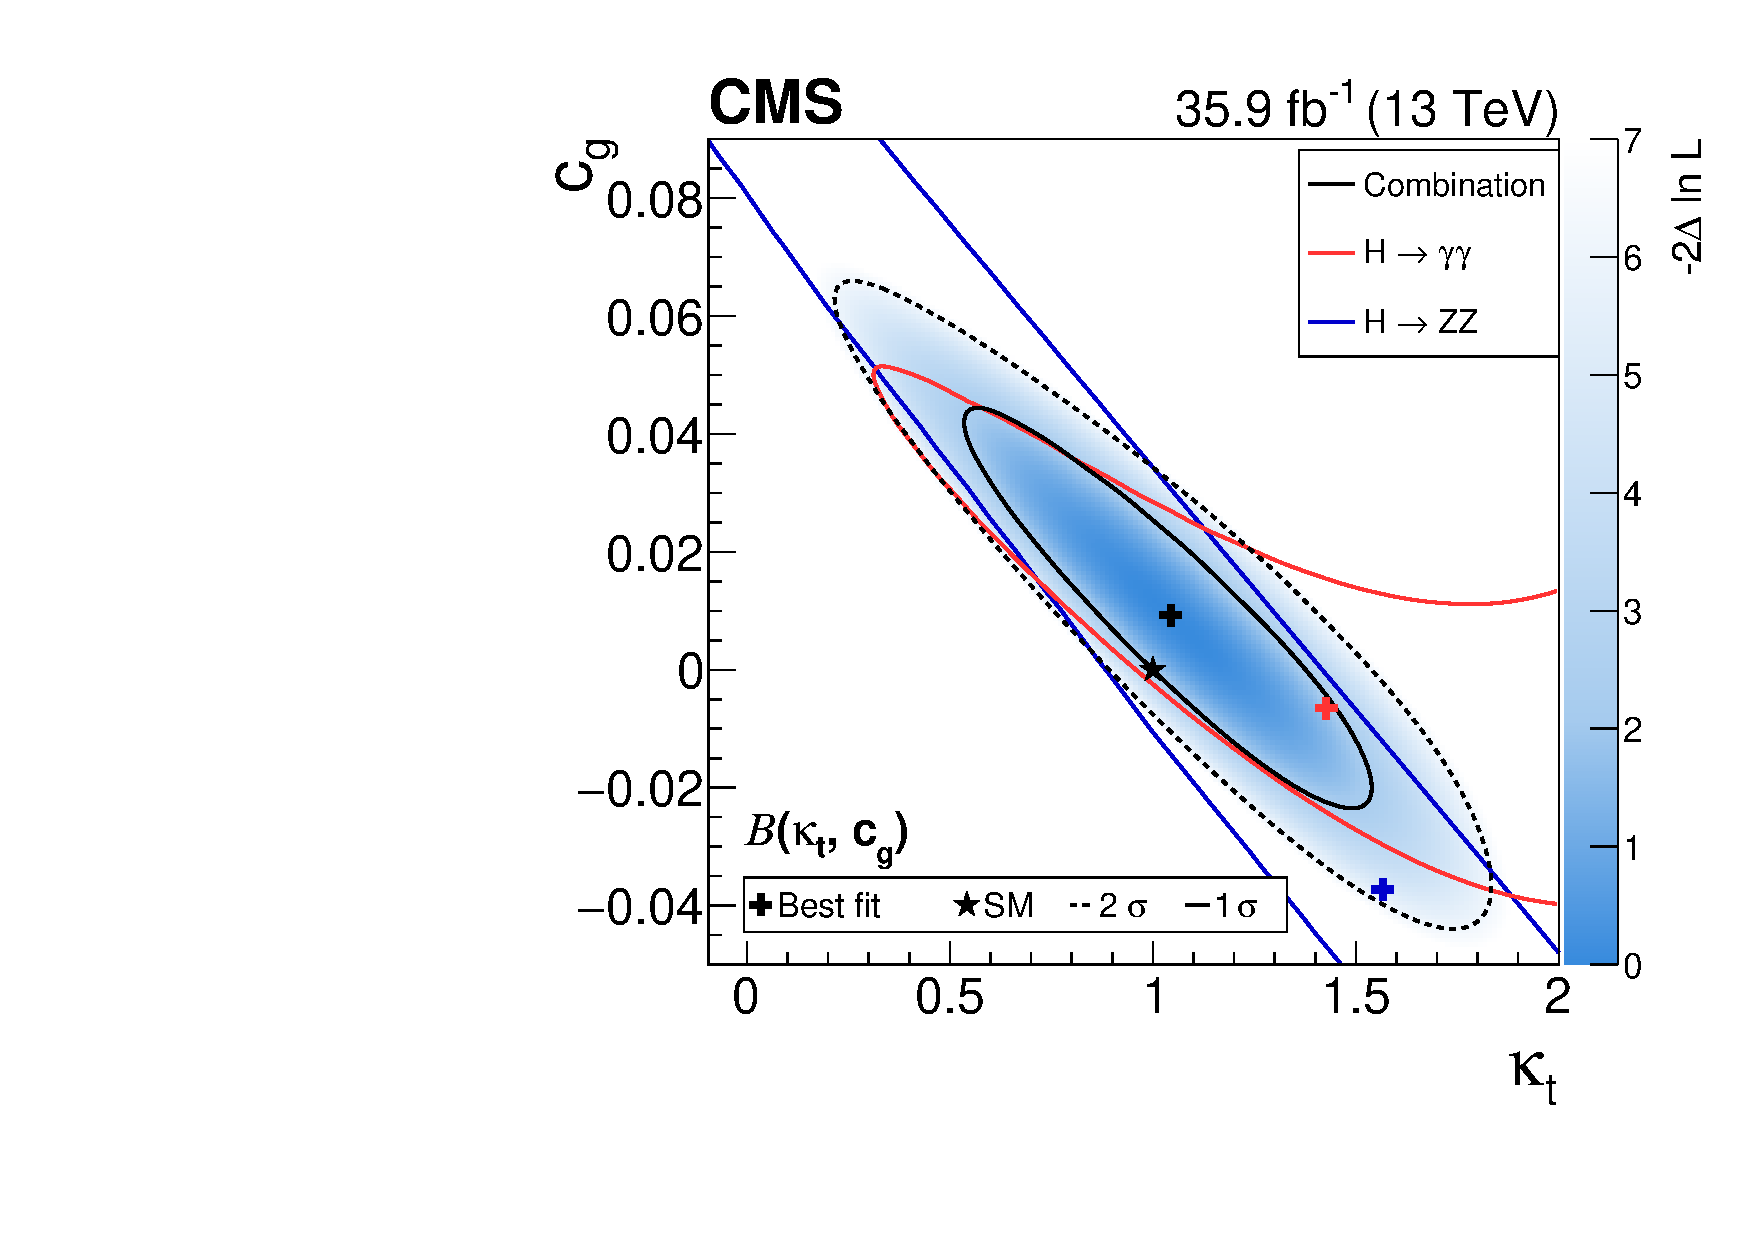
\includegraphics[width=0.49\linewidth]{img/interpretation/multicont_ktcg_couplingdependentBRs.pdf}
        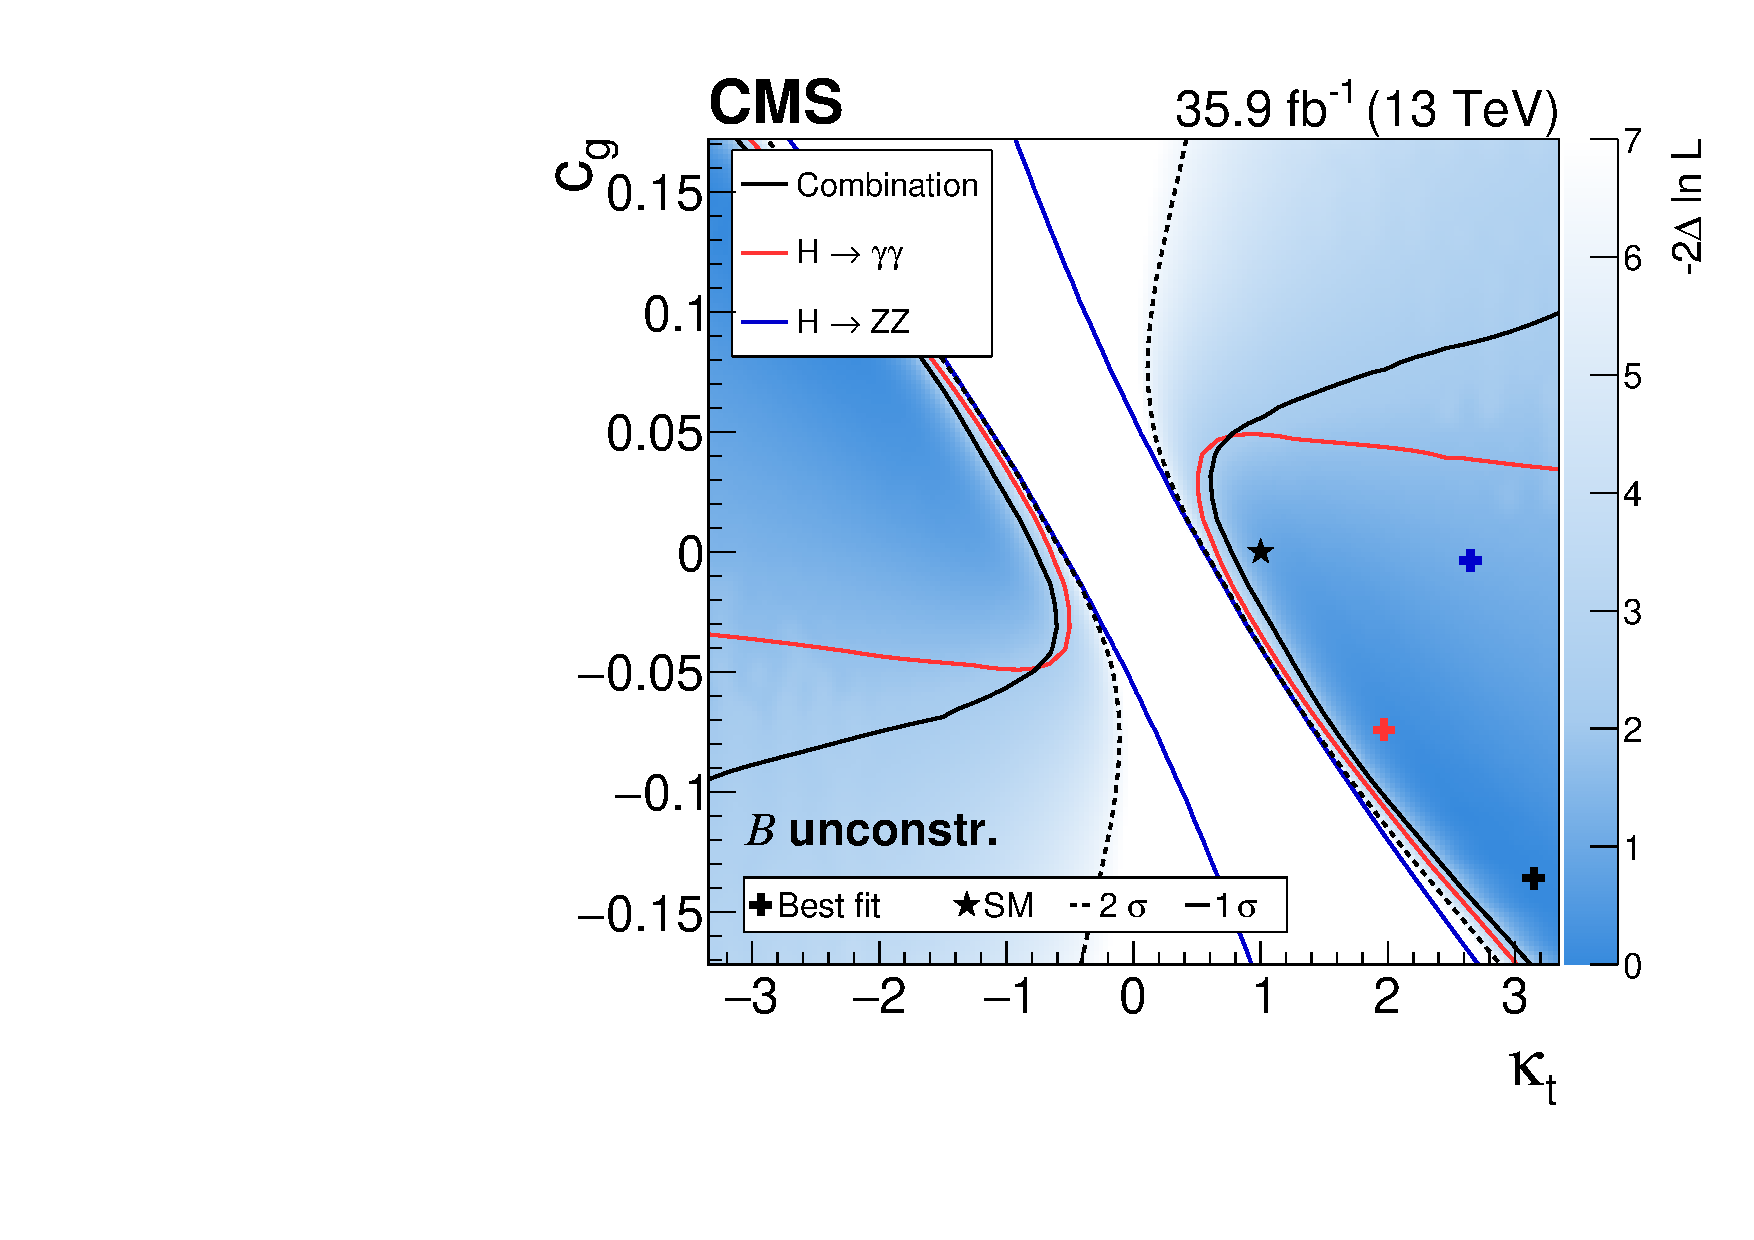
\includegraphics[width=0.49\linewidth]{img/interpretation/multicont_ktcg_floatingBRs.pdf}        
        }
    % 
    \caption{
        Simultaneous fit to data for $\kappat$ and $\cg$, assuming a coupling dependence of the branching fractions (left) and the branching fractions implemented as nuisance parameters with no prior constraint (right).
        % 
        The one standard deviation contour is drawn for the combination ($\hgg$, $\hzz$, and $\hbb$), the $\hgg$ channel, and the $\hzz$ channel in black, red, and blue, respectively.
        % 
        For the combination the two standard deviation contour is drawn as a black dashed line, and the shading indicates the negative log-likelihood, with the scale shown on the right hand side of the plots.
        }
    \label{fig:scans_kappatkappag_nominal}
  \end{center}
\end{figure}


Figure~\ref{fig:scans_kappatkappab_rawInput} (left) shows the combined log-likelihood scan as a function of $\kappat$ and $\kappab$, with branching fractions scaling appropriately with the coupling modifiers and Figure~\ref{fig:scans_kappatkappab_rawInput} (right) with the branching fractions implemented as nuisance parameters with no prior constraint.
% 
As the $\hgg$ branching fraction depends linearly on $\kappat$, the constraints on the $\hgg$ channel and the combination in Figure~\ref{fig:scans_kappatkappab_rawInput} (left) are not symmetric with respect to the $\kappat$ axis.
% 
For the branching fractions implemented as nuisance parameters with no prior constraint, the parametrization is symmetric under $(\kappat,\,\kappab) \, \to \, (-\kappat,\,-\kappab)$, which explains the observed symmetry in Figure~\ref{fig:scans_kappatkappab_rawInput} (right).

\begin{figure}[hbtp]
  \begin{center}
    \ifbool{draftmode}{
        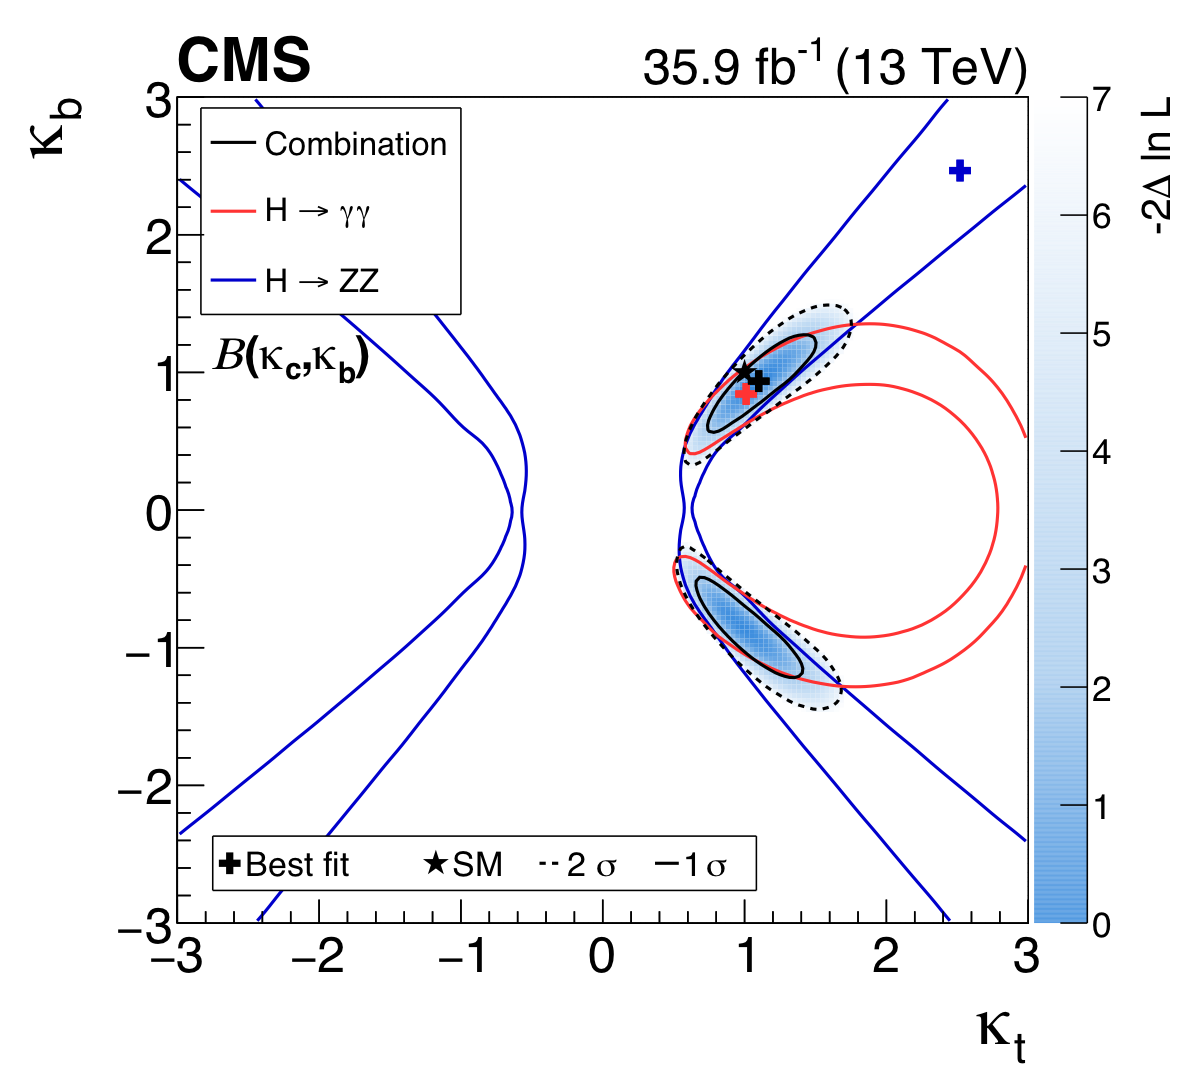
\includegraphics[width=0.49\linewidth]{img/interpretation/multicont_ktkb_couplingdependentBRs.png}
        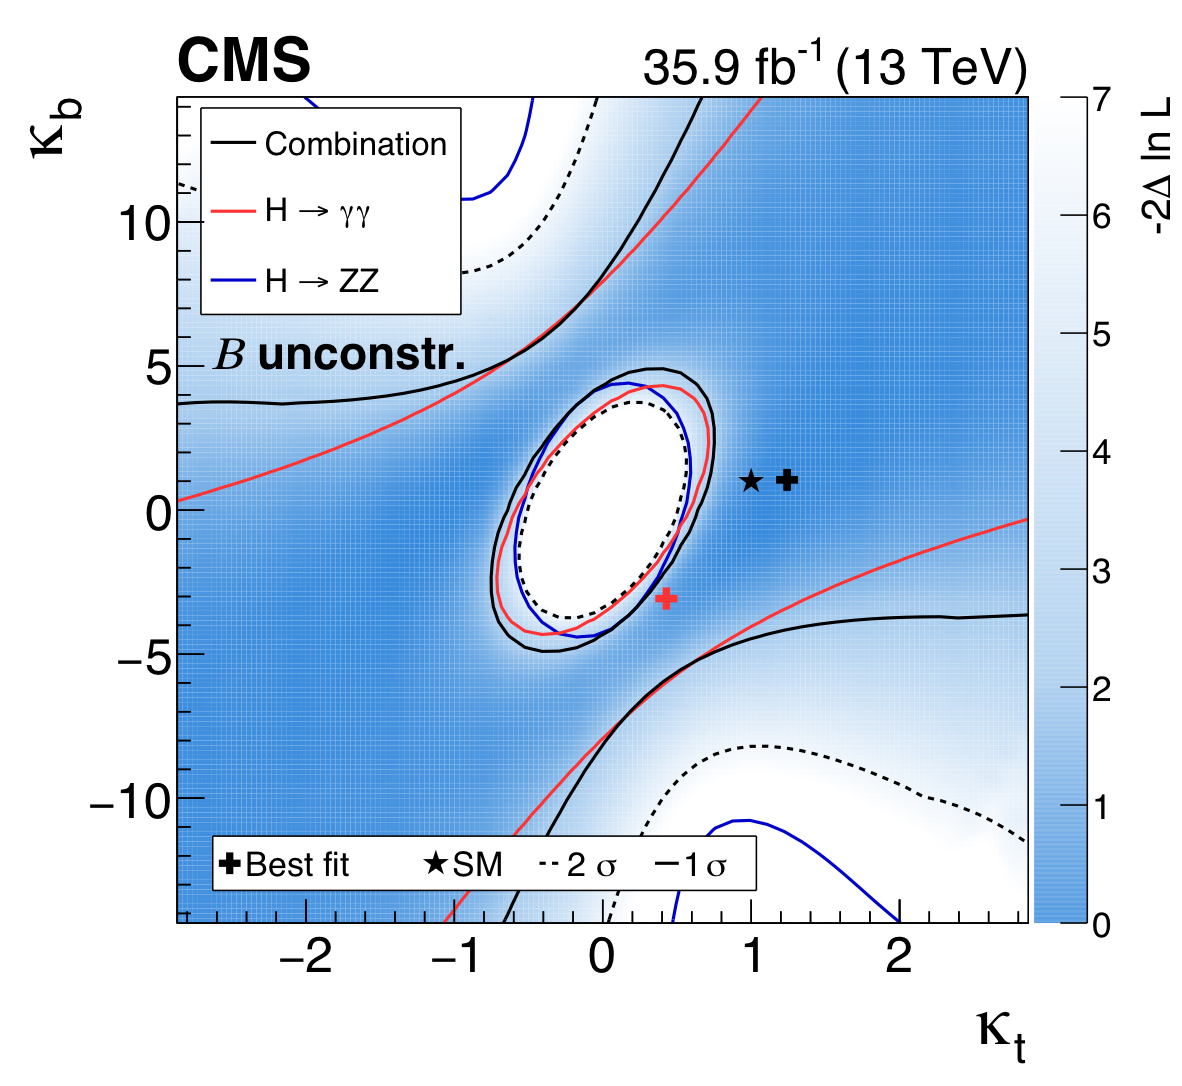
\includegraphics[width=0.49\linewidth]{img/interpretation/multicont_ktkb_floatingBRs.png}
        }{
        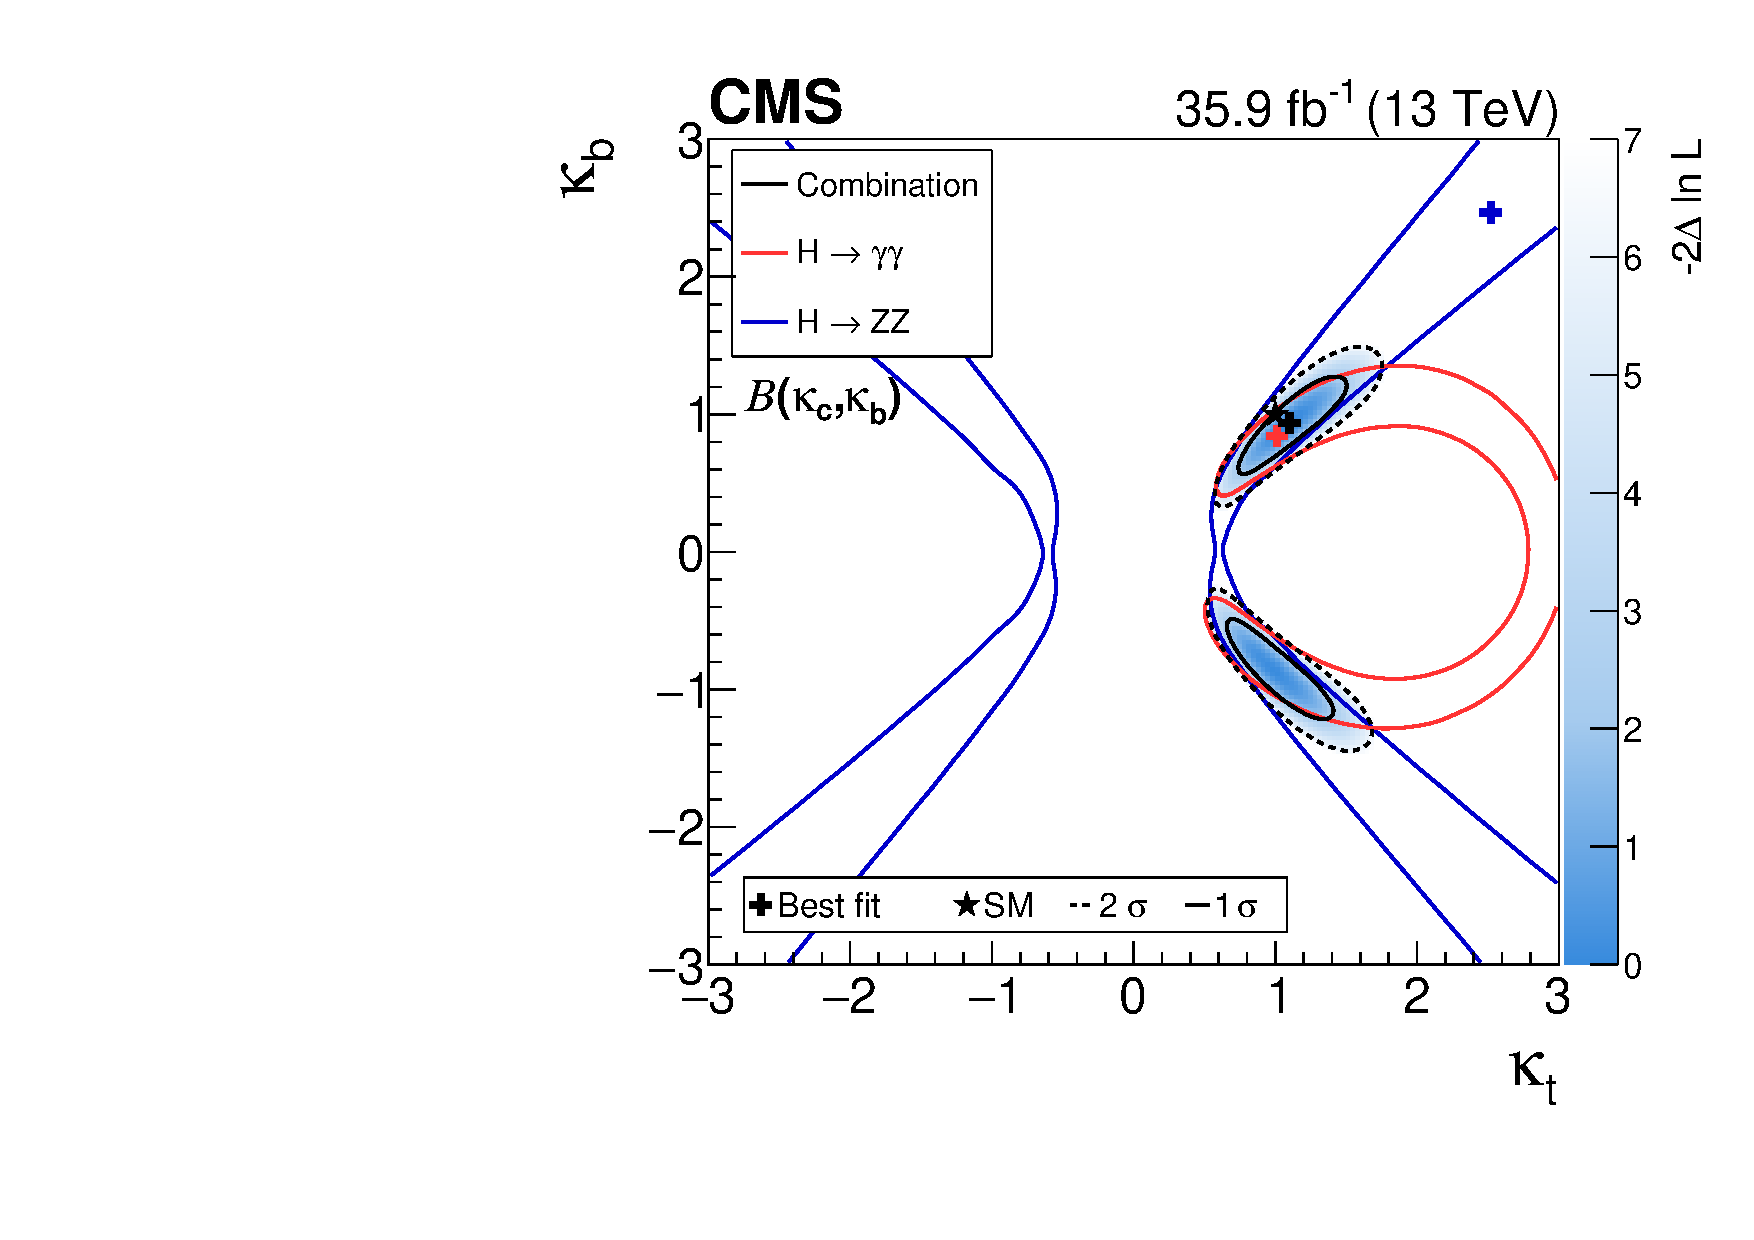
\includegraphics[width=0.49\linewidth]{img/interpretation/multicont_ktkb_couplingdependentBRs.pdf}
        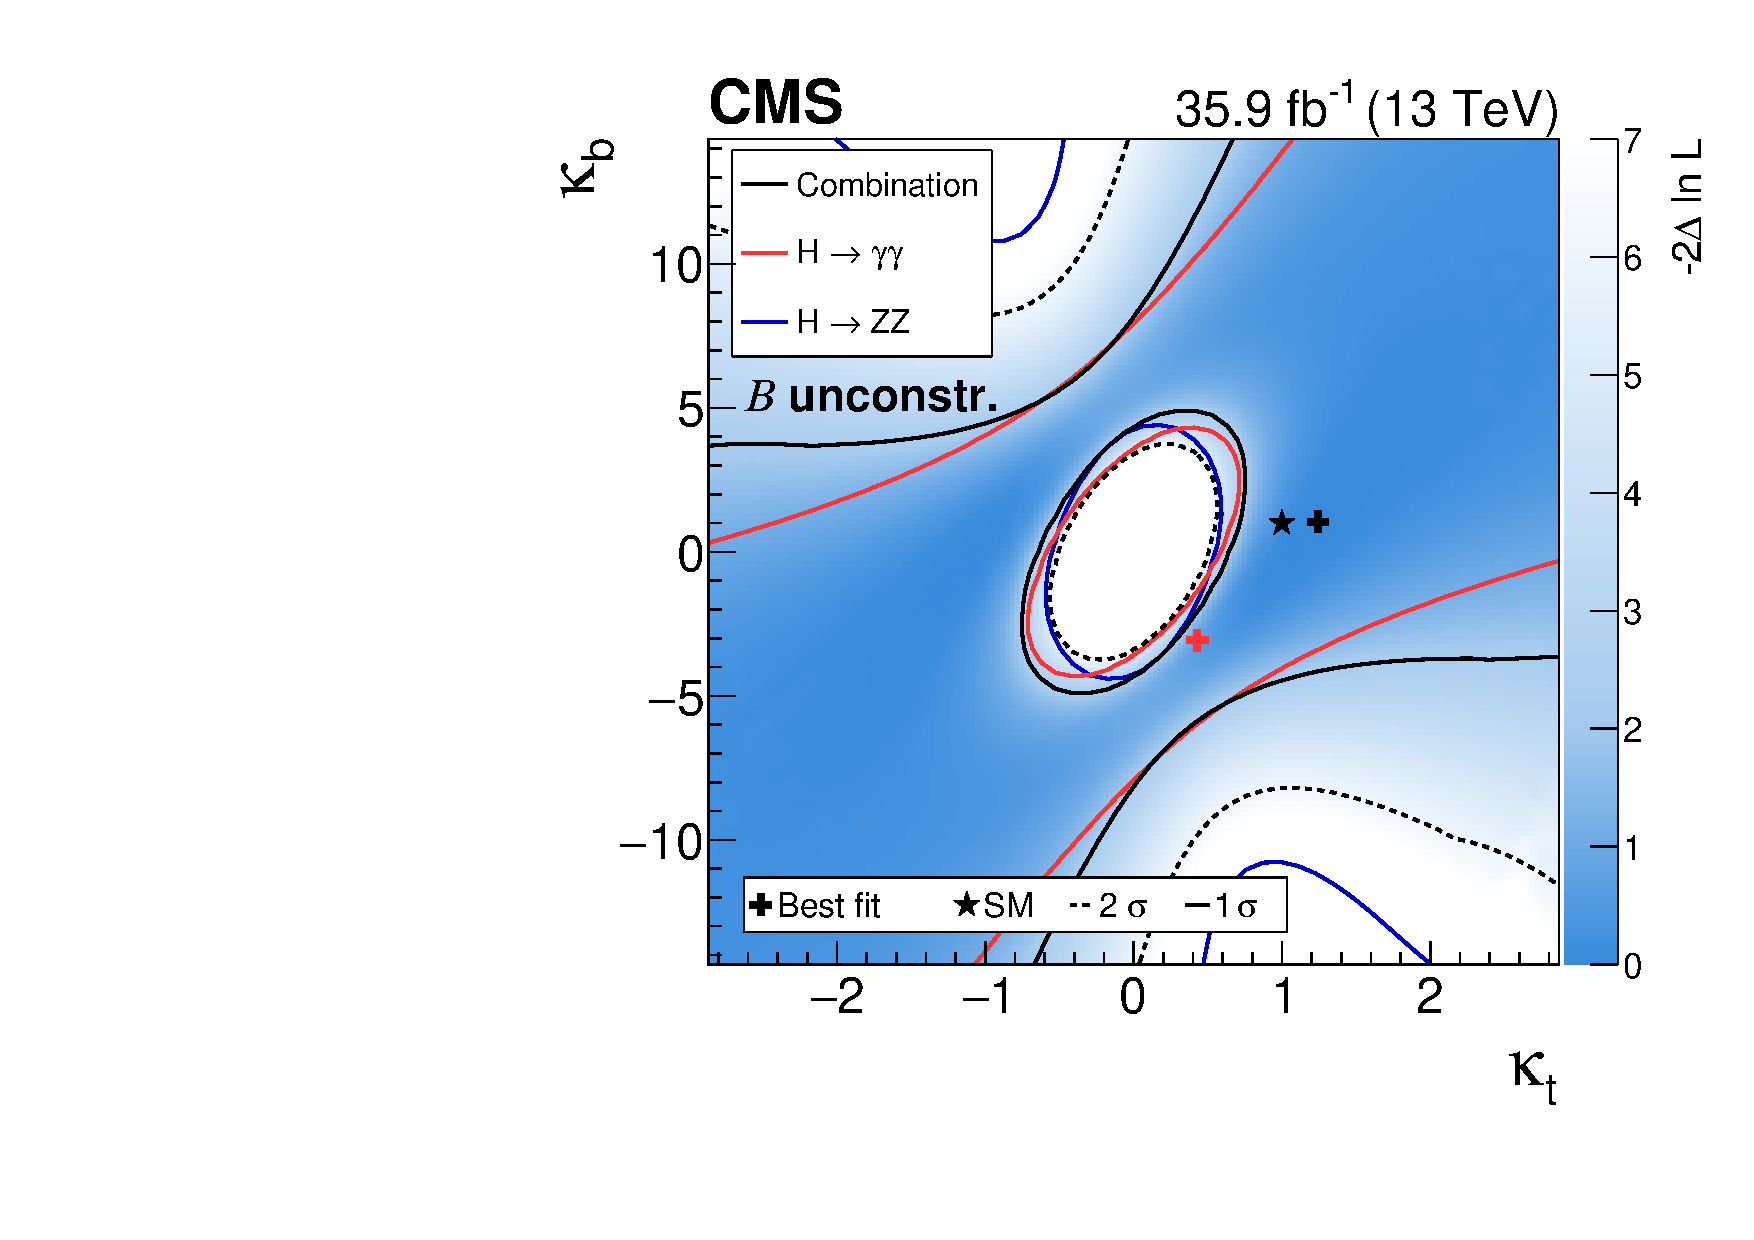
\includegraphics[width=0.49\linewidth]{img/interpretation/multicont_ktkb_floatingBRs.pdf}        
        }
    % 
    \caption{
        Simultaneous fit to data for $\kappat$ and $\kappab$, assuming a coupling dependence of the branching fractions (left) and the branching fractions implemented as nuisance parameters with no prior constraint (right).
        % 
        The one standard deviation contour is drawn for the combination ($\hgg$, $\hzz$, and $\hbb$), the $\hgg$ channel, and the $\hzz$ channel in black, red, and blue, respectively.
        % 
        For the combination the two standard deviation contour is drawn as a black dashed line, and the shading indicates the negative log-likelihood, with the scale shown on the right hand side of the plots.
        }
    \label{fig:scans_kappatkappab_rawInput}
  \end{center}
\end{figure}





% ____________________________________________________________________________
\subsection{Simultaneous variations of \texorpdfstring{$\kappab$}{kb} and \texorpdfstring{$\kappac$}{kc}}

\tk{TODO:
Introduction of the theory, results when fitting it to data.
}

\subsubsection{Results}

\tk{TODO: Literal copy from paper now}

Figure~\ref{fig:scans_kappabkappac_nominal} (left) shows the one and two standard deviation contours of the fits of the $\kappab/\kappac$ parametrization from Ref.~\cite{Bishara:2016jga} to data, assuming the branching fractions are dependent on the Higgs boson couplings, i.e., $\mathcal{B} = \mathcal{B}(\kappab, \kappac)$, and that there are no beyond-the-SM contributions.
% 
The substructure on the combined scan shows a ring shape around the origin, in agreement with the SM prediction within one standard deviation.


The fit is repeated with the branching fractions for the $\hgg$ and $\hzz$ channels implemented as nuisance parameters with no prior constraint, effectively removing dependence from the total width and the overall normalization.
% 
This way the constraint on $\kappab$ and $\kappac$ comes only from the knowledge of the $\pth$ distribution.
% distortion of the normalized $\pth$ spectrum.
% 
The result of this fit is shown in Fig.~\ref{fig:scans_kappabkappac_nominal} (right).
% 
As expected, the range of allowed values of $\kappab$ and $\kappac$ is much wider than in the case of coupling-dependent branching fractions.

\begin{figure}[hbtp]
  \begin{center}
    \ifbool{draftmode}{
        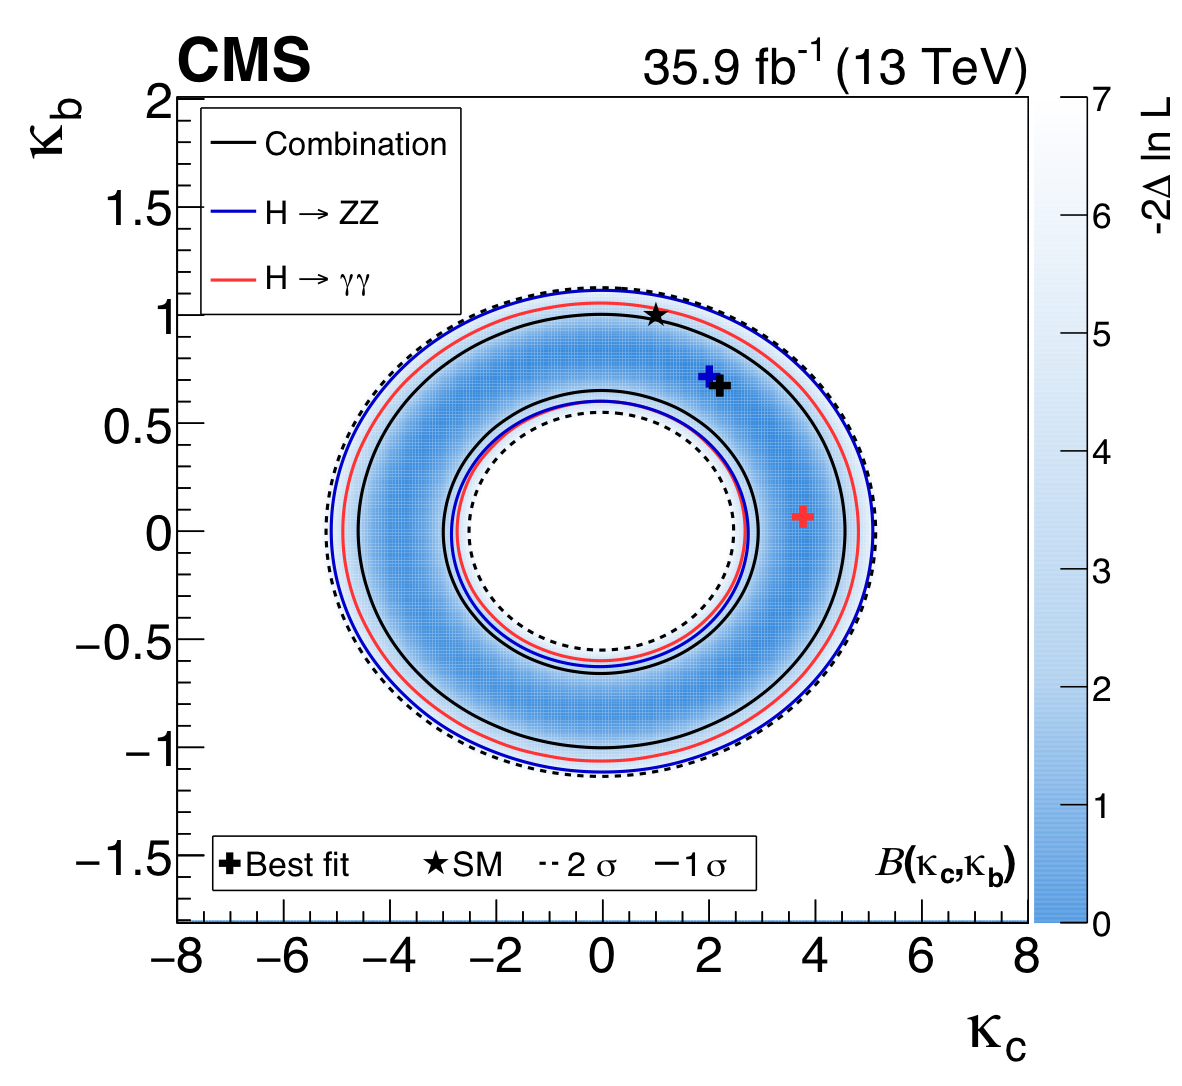
\includegraphics[width=0.49\linewidth]{img/interpretation/multicont_Yukawa_couplingdependentBRs.png}
        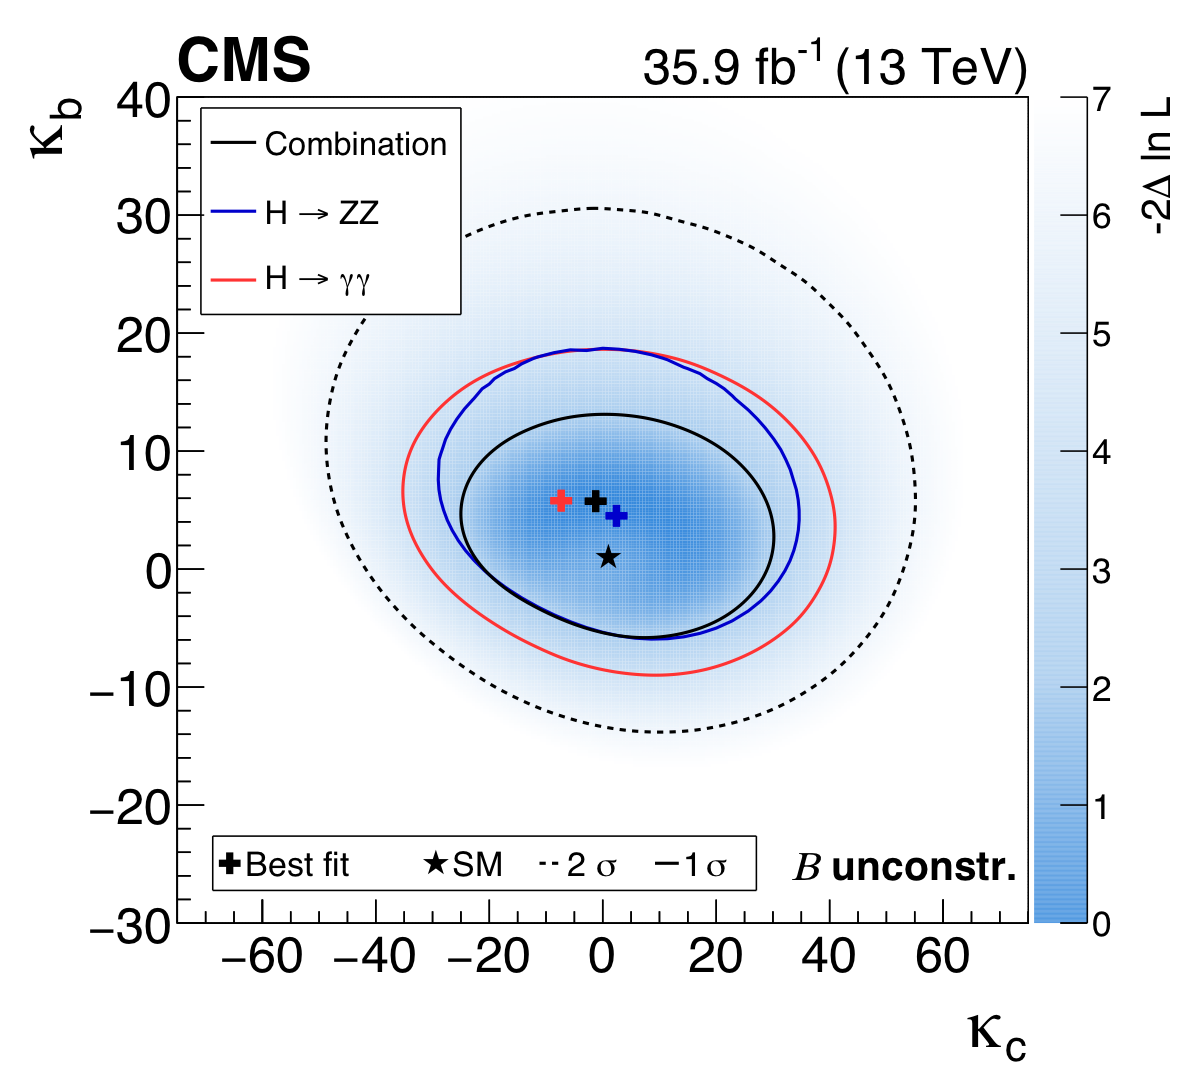
\includegraphics[width=0.49\linewidth]{img/interpretation/multicont_Yukawa_floatingBRs.png}
        }{
        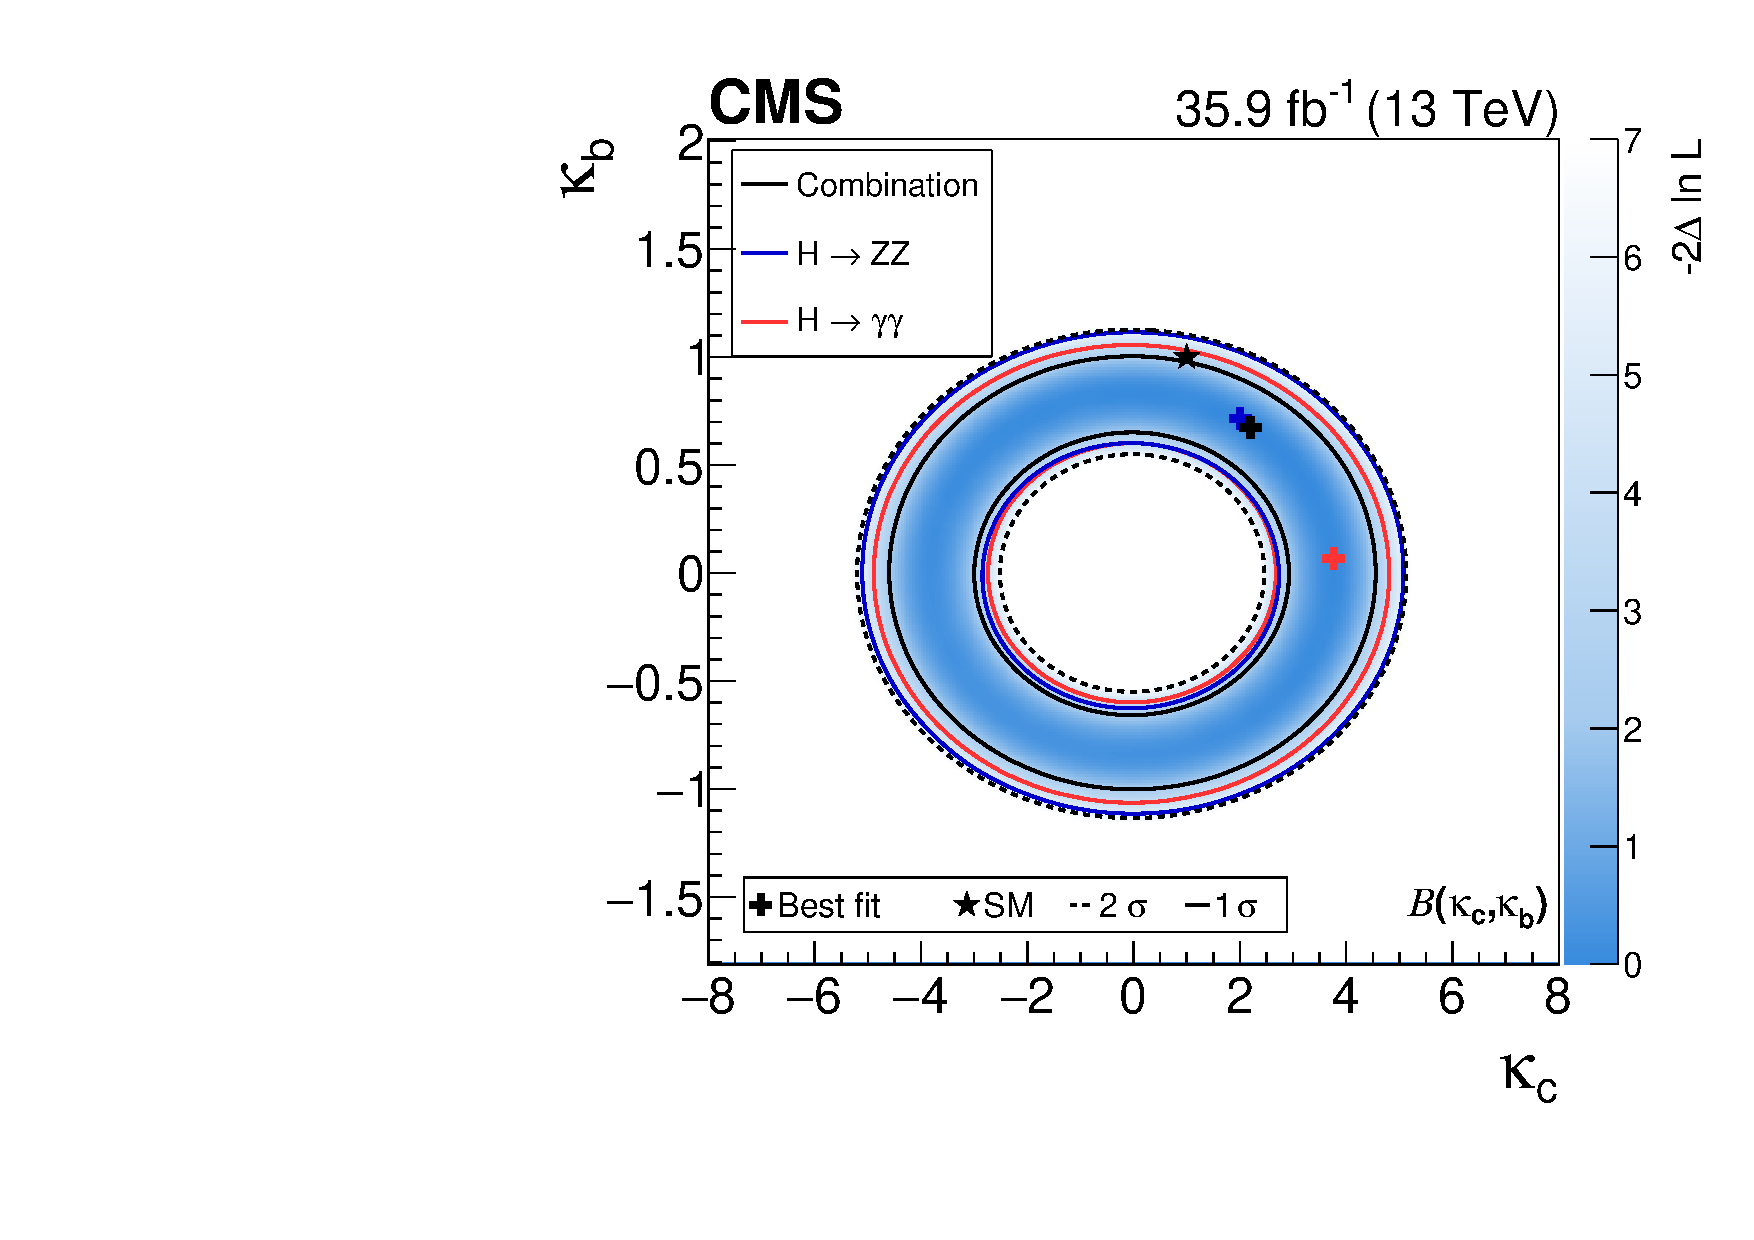
\includegraphics[width=0.49\linewidth]{img/interpretation/multicont_Yukawa_couplingdependentBRs.pdf}
        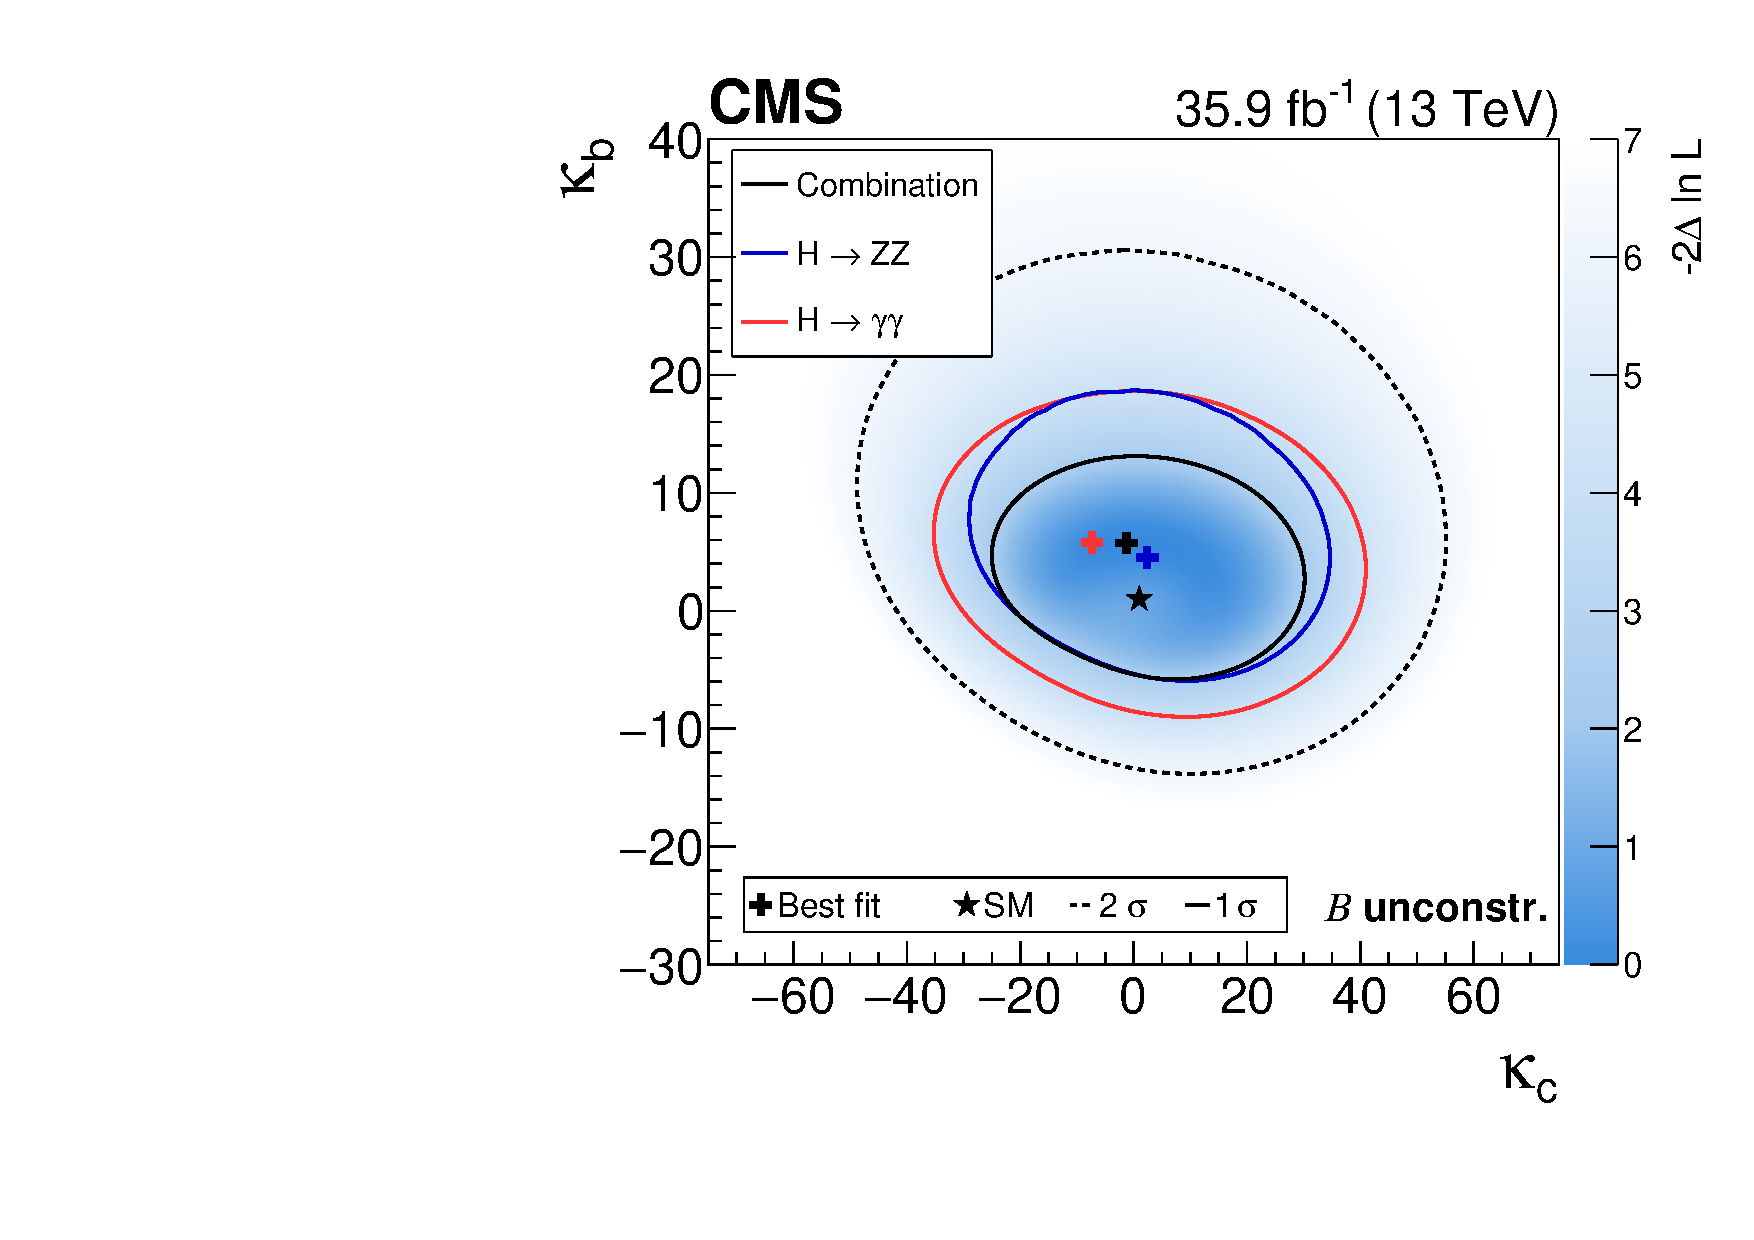
\includegraphics[width=0.49\linewidth]{img/interpretation/multicont_Yukawa_floatingBRs.pdf}        
        }
    % 
    \caption{
        Simultaneous fit to data for $\kappab$ and $\kappac$, assuming a coupling dependence of the branching fractions (left) and the branching fractions implemented as nuisance parameters with no prior constraint (right).
        % 
        The one standard deviation contour is drawn for the combination ($\hgg$ and $\hzz$), the $\hgg$ channel, and the $\hzz$ channel in black, red, and blue, respectively.
        % 
        For the combination the two standard deviation contour is drawn as a black dashed line, and the shading indicates the negative log-likelihood, with the scale shown on the right hand side of the plots.
        }
    \label{fig:scans_kappabkappac_nominal}
  \end{center}
\end{figure}


Confidence intervals can be set on $\kappab$ and $\kappac$ by profiling one coupling and scanning over the other.
% 
The results of these single-coupling scans are shown in Fig.~\ref{fig:scans_kappabkappac_oneDimScans} and \ref{fig:scans_kappabkappac_oneDimScans_scenario2}.
% 
The observed (expected) limits at 95\% CL in the one-dimensional scans are:
% 
% \clearpage
\begin{linenomath*}
\begin{equation}
\label{eq:kappasensitivity}
\begin{array}{c}
\kappabLeftObserved < \kappab < \kappabRightObserved  \quad(\kappabLeftAsimov < \kappab < \kappabRightAsimov )  \,,
\\[8pt]
\kappacLeftObserved < \kappac < \kappacRightObserved \quad(\kappacLeftAsimov < \kappac < \kappacRightAsimov )
\,,
\end{array}
\end{equation}
\end{linenomath*}
% 
in the case of branching fractions that depend on $\kappab$ and $\kappac$, and
% 
\begin{linenomath*}
\begin{equation}
\label{eq:kappasensitivity_floatingBRs}
\begin{array}{c}
\kappabLeftObservedFLOATINGBRS < \kappab < \kappabRightObservedFLOATINGBRS  \quad(\kappabLeftAsimovFLOATINGBRS < \kappab < \kappabRightAsimovFLOATINGBRS )  \,,
\\[8pt]
\kappacLeftObservedFLOATINGBRS < \kappac < \kappacRightObservedFLOATINGBRS \quad(\kappacLeftAsimovFLOATINGBRS < \kappac < \kappacRightAsimovFLOATINGBRS )
\,,
\end{array}
\end{equation}
\end{linenomath*}
% 
in the case of the branching fractions implemented as nuisance parameters with no prior constraint.
% 
For the coupling-dependent branching fractions, the results are shaped predominantly by the constraints from the total width rather than by distortions of the $\pth$ spectrum.
% 
If the branching fractions are fixed to their SM expectations, the one-dimensional scans yield the following expected limits at 95\% CL:
% 
\begin{linenomath*}
\begin{equation}
\label{eq:kappasensitivity_fixedSMBRs}
\begin{array}{c}
-3.5 < \kappab < 5.1  \,,
 \\[8pt]
-13 < \kappac < 15
\,.
\end{array}
\end{equation}
\end{linenomath*}
% 
These intervals are comparable to those in Ref.~\cite{Bishara:2016jga}, where $\kappac \in [ -16, 18 ]$ at 95\% CL, noting that the results here are based on a larger data set.
% 
The intervals obtained are competitive with the intervals from other direct search channels summarized in Section~\ref{sec:introduction}.


\begin{figure}[hbtp]
  \begin{center}
    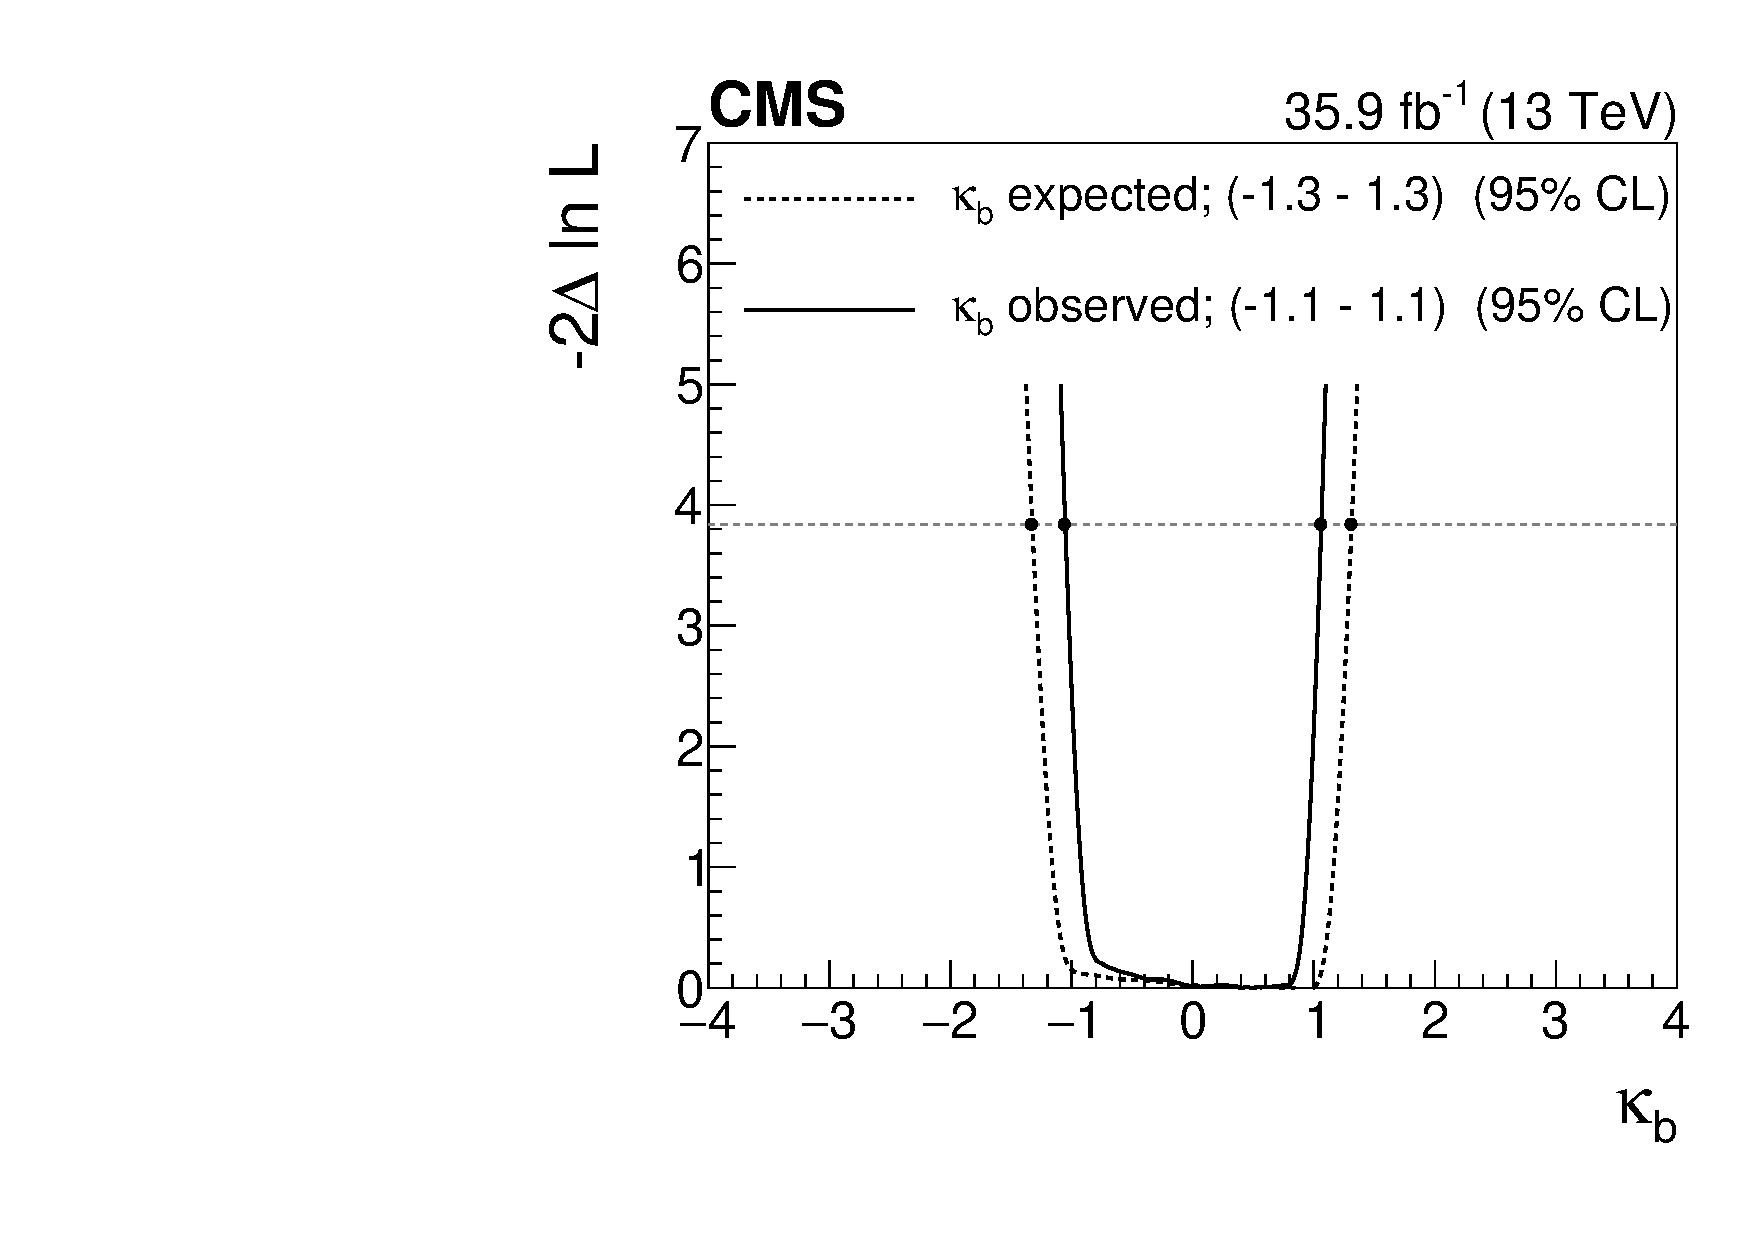
\includegraphics[width=0.49\linewidth]{img/interpretation/onekappascan_kbkc_couplingdependentBRs_kappab.pdf}
    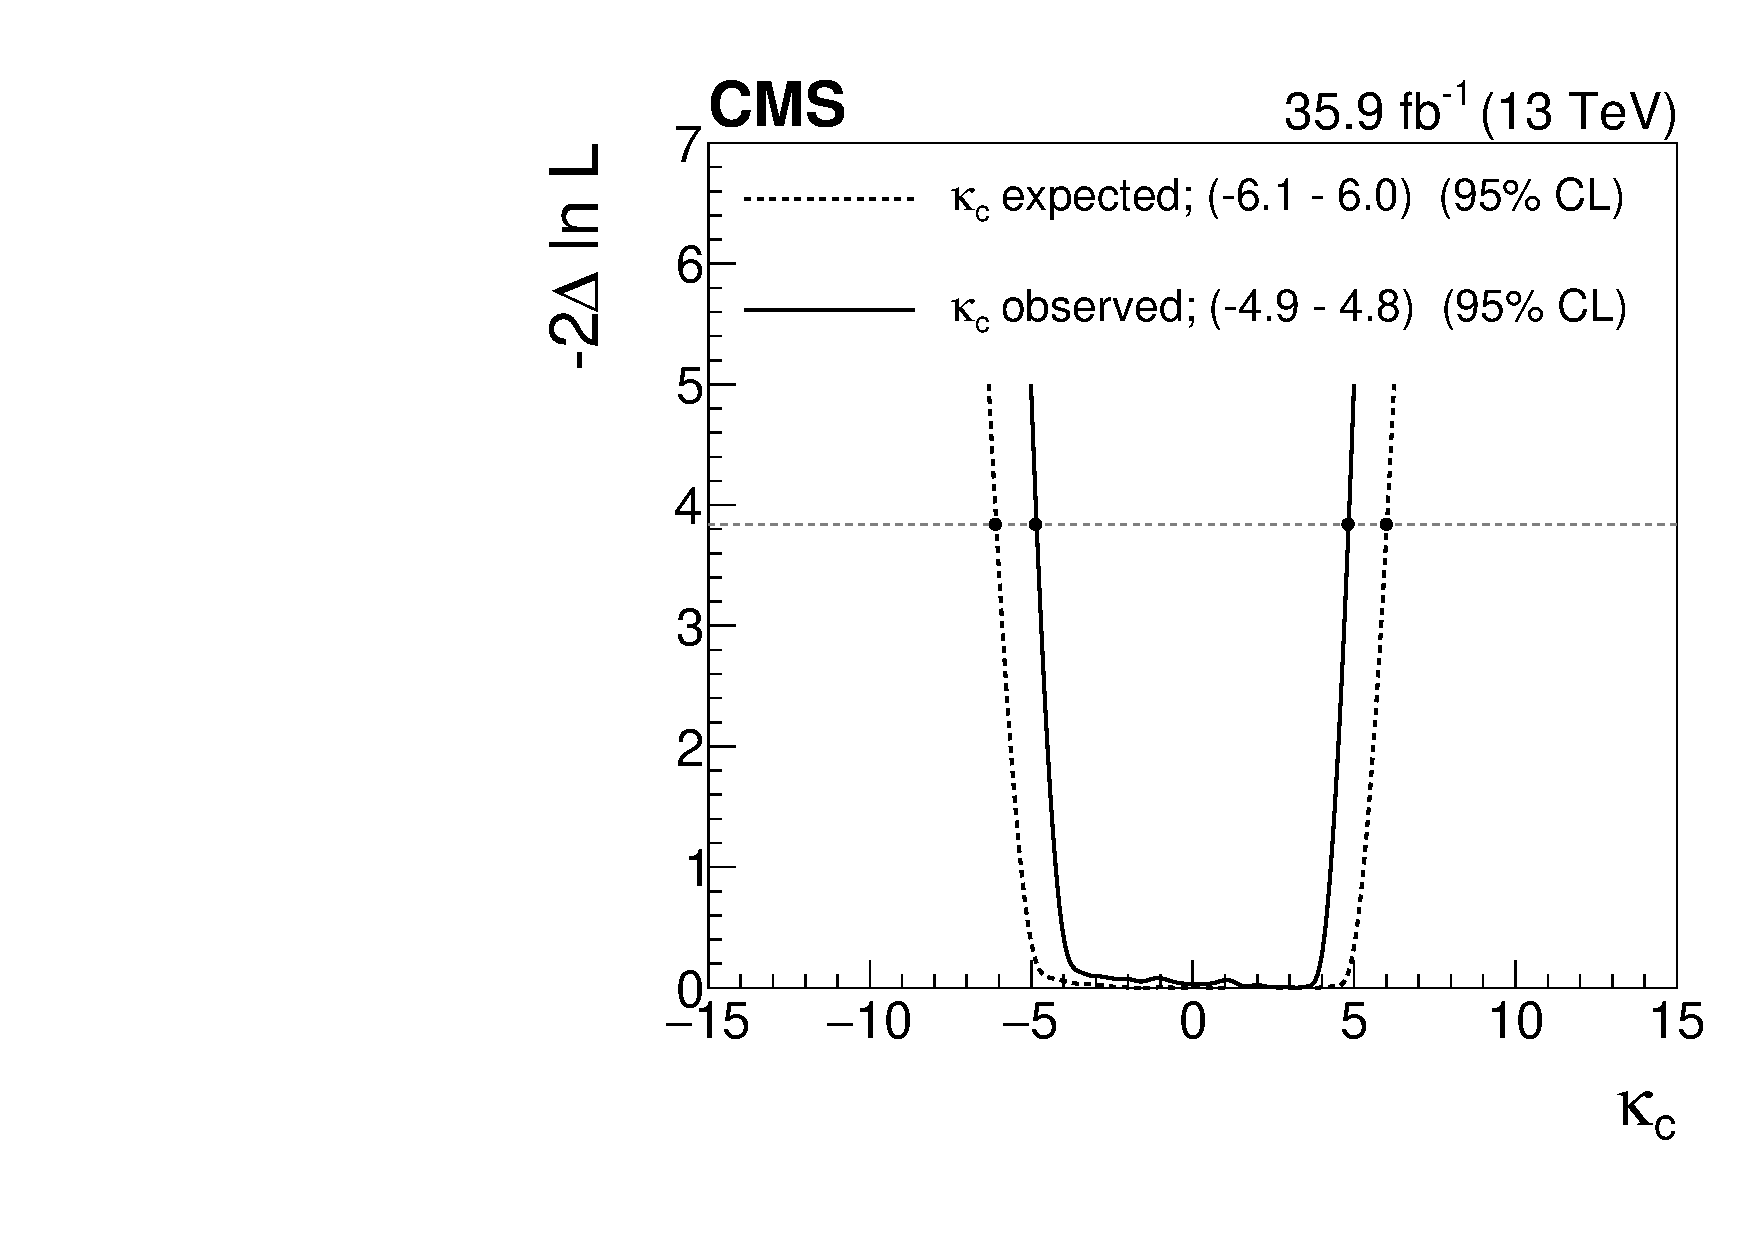
\includegraphics[width=0.49\linewidth]{img/interpretation/onekappascan_kbkc_couplingdependentBRs_kappac.pdf}
    \caption{
        Likelihood scan of $\kappab$ while profiling $\kappac$ (left), and of $\kappac$ while profiling $\kappab$ (right).
        % 
        The filled markers indicate the limits at 95\% CL.
        % 
        The branching fractions are considered dependent on the values of the couplings.
        }
    \label{fig:scans_kappabkappac_oneDimScans}
  \end{center}
\end{figure}

\begin{figure}[hbtp]
  \begin{center}
    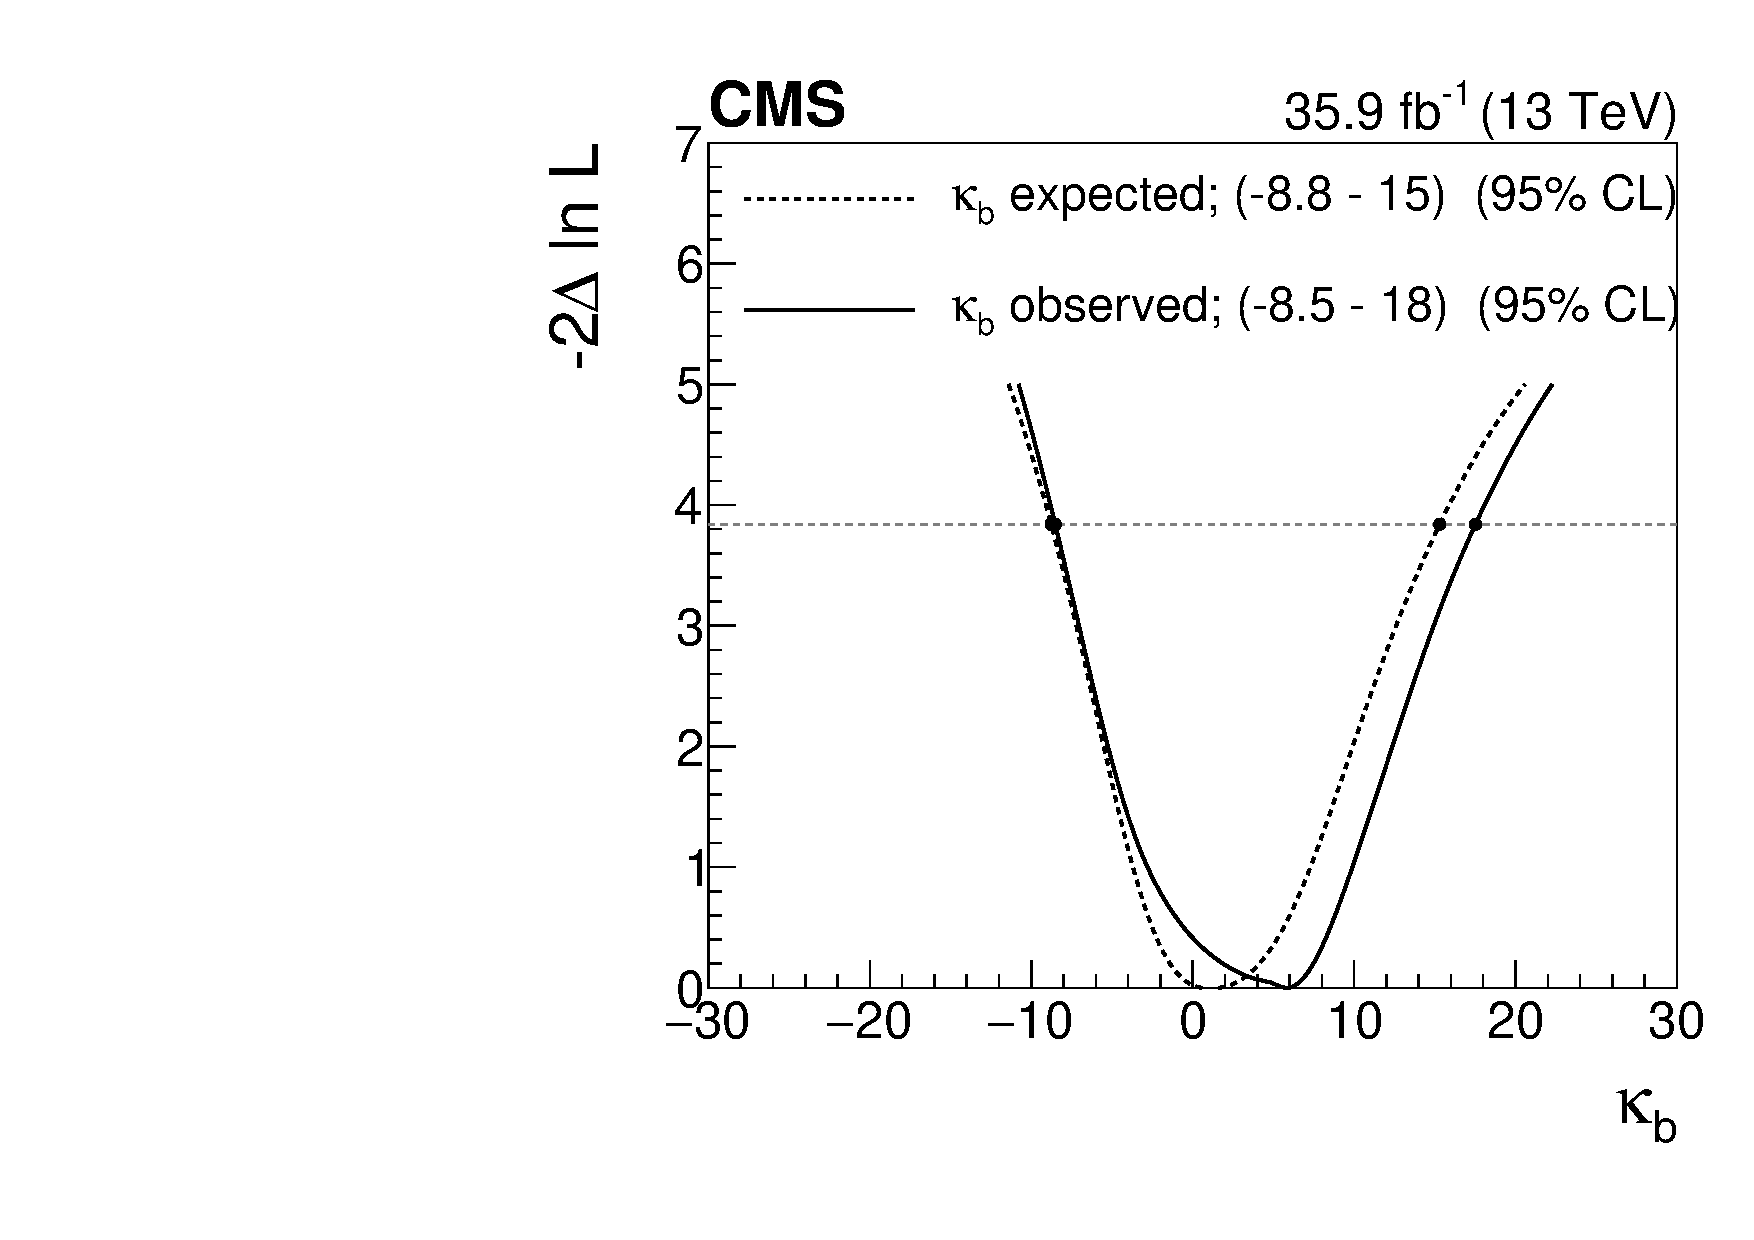
\includegraphics[width=0.49\linewidth]{img/interpretation/onekappascan_kbkc_floatingBRs_kappab.pdf}
    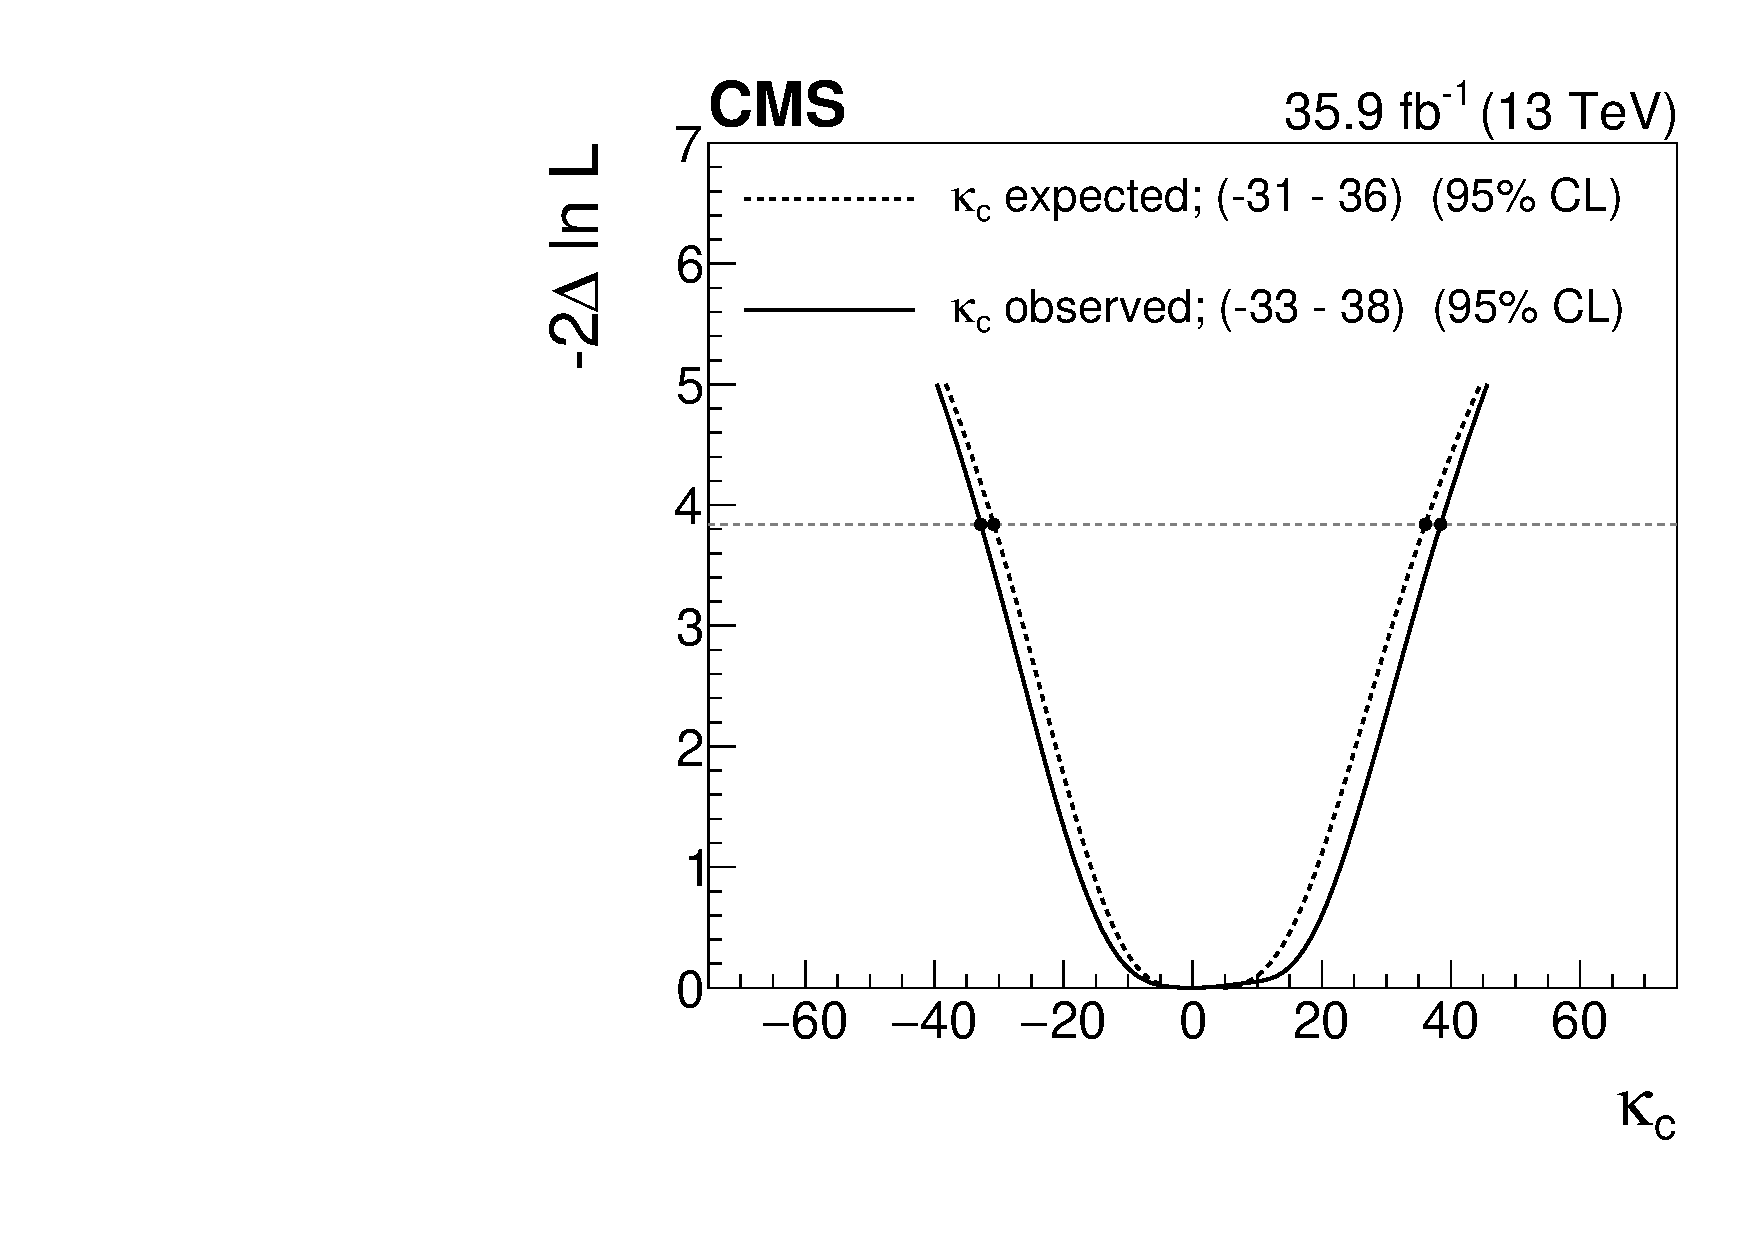
\includegraphics[width=0.49\linewidth]{img/interpretation/onekappascan_kbkc_floatingBRs_kappac.pdf}
    \caption{
        Likelihood scan of $\kappab$ while profiling $\kappac$ (left), and of $\kappac$ while profiling $\kappab$ (right).
        % 
        The filled markers indicate the limits at 95\% CL.
        % 
        The branching fractions are implemented as nuisance parameters with no prior constraint.
        }
    \label{fig:scans_kappabkappac_oneDimScans_scenario2}
  \end{center}
\end{figure}

